%%%%%%%%%%%%%%%%%%%%%%%%%%%%%%%%%%%%%%%%%%%%%%%%%%%%%%%%%%%%%%%%%%%%%%%%%%%
% BSc (Hons) AI & Data Science — Individual Research Project Thesis
% Dynamic Narrative Personalization in Games Using AI
% Rivindu Bopage — RGU 2312553 / IIT 20220580
%%%%%%%%%%%%%%%%%%%%%%%%%%%%%%%%%%%%%%%%%%%%%%%%%%%%%%%%%%%%%%%%%%%%%%%%%%%
\documentclass[12pt,a4paper]{report}

% -- Packages --
\usepackage[a4paper,margin=1in]{geometry}
\usepackage{setspace}
\usepackage{graphicx}
\usepackage{titlesec}
\usepackage{tocloft}
\usepackage{fancyhdr}
\usepackage{natbib}
\usepackage{threeparttable}
\usepackage{xurl}
\usepackage{array}
\usepackage{float}
\usepackage{multirow}
\usepackage{amsmath}
\usepackage{booktabs}
\usepackage{etoolbox}
\usepackage{hyperref}
\usepackage{url}
\usepackage{enumitem}
\usepackage{tcolorbox}
\usepackage{listings}
\usepackage[utf8]{inputenc}
\usepackage[T1]{fontenc}
\usepackage{subcaption}
\usepackage{pdfpages}
\usepackage{longtable}
\usepackage{tabularx}
\usepackage{tikz}
\usetikzlibrary{arrows.meta, positioning, shapes.geometric, fit, backgrounds, calc, decorations.markings}
\usepackage{pgfgantt}
\usepackage{pgfplots}
\pgfplotsset{compat=1.18}

\lstset{inputencoding=utf8, extendedchars=true, basicstyle=\ttfamily\small, breaklines=true, frame=single}

\makeatletter
\patchcmd{\maketitle}{\vskip 0.5em}{\vskip -0.5em}{}{}
\makeatother

% -- Font: Times New Roman --
\usepackage{mathptmx}

% -- Header & Footer --
\pagestyle{fancy}
\fancyhf{}
\renewcommand{\headrulewidth}{0pt}
\cfoot{\thepage}

% -- Chapter formatting --
\titleformat{\chapter}[display]
  {\normalfont\large\centering}
  {\itshape\chaptertitlename\ \thechapter}
  {10pt}
  {\uppercase}
\titlespacing*{\chapter}{0pt}{0pt}{25pt}

% -- TOC / LOF / LOT titles to match chapter style (uppercase, centered) --
\renewcommand{\contentsname}{\uppercase{Contents}}
\renewcommand{\listfigurename}{\uppercase{List of Figures}}
\renewcommand{\listtablename}{\uppercase{List of Tables}}
\renewcommand{\cfttoctitlefont}{\hfill\normalfont\large}
\renewcommand{\cftaftertoctitle}{\hfill}
\renewcommand{\cftloftitlefont}{\hfill\normalfont\large}
\renewcommand{\cftafterloftitle}{\hfill}
\renewcommand{\cftlottitlefont}{\hfill\normalfont\large}
\renewcommand{\cftafterlottitle}{\hfill}
\setlength{\cftbeforetoctitleskip}{0pt}
\setlength{\cftbeforeloftitleskip}{0pt}
\setlength{\cftbeforelottitleskip}{0pt}
\setlength{\cftaftertoctitleskip}{25pt}
\setlength{\cftafterloftitleskip}{25pt}
\setlength{\cftafterlottitleskip}{25pt}

% -- Section formatting --
\titleformat{\section}
  {\normalfont\large\bfseries}
  {\thesection}{1em}{}

\titleformat{\subsection}
  {\normalfont\normalsize\bfseries}
  {\thesubsection}{1em}{}

% -- Line Spacing --
\onehalfspacing
\setlength{\parindent}{15pt}
\setlength{\parskip}{0pt}

% -- Hyperref setup --
\hypersetup{
  colorlinks=true,
  linkcolor=black,
  citecolor=black,
  urlcolor=blue
}

% -- Abbreviation table helper --
\newcommand{\abbrev}[2]{\textbf{#1} & #2 \\}

%==========================================================================
\begin{document}

% --- Front matter ---
%--------------------------------------------------------------------------
% TITLE PAGE
%--------------------------------------------------------------------------
\begin{titlepage}
\centering


\includegraphics[height=1.5cm]{TitleFigs/rgu_logo.jpg}\hspace{3cm}

\includegraphics[height=1.5cm, width=4cm]{TitleFigs/iit_logo.png}

\vspace{1.6cm}

{\Large \textbf{Informatics Institute of Technology}}

\vspace{0.4cm}

{\large In Collaboration with}

\vspace{0.4cm}

{\Large \textbf{Robert Gordon University, Aberdeen, Scotland}}

\vspace{2cm}

{\Large\bfseries
AI-Driven Dynamic Narrative Personalization in Games:\\[6pt]
A Closed-Loop Plugin Using Hexad Player Modeling,\\[6pt]
RAG-Grounded LLM Generation, and PPO Reinforcement Learning
}

\vspace{1.5cm}

{\Large Final Year Thesis by}

\vspace{0.4cm}

{\Large \textbf{Rivindu Bopage}}

\vspace{1cm}

{\small RGU ID -- 2312553}\\
{\small IIT ID -- 20220580}

\vspace{1cm}

{\Large Supervised by}

\vspace{0.4cm}

{\large \textbf{Bimali Wickramasinghe}}

\vspace{1cm}

{\large April 2026}

\vfill

\small
Submitted in partial fulfilment of the requirements for the\\
BSc.\ (Hons) in Artificial Intelligence and Data Science at the Robert Gordon University, Aberdeen, UK.

\end{titlepage}

%--------------------------------------------------------------------------
% FRONT MATTER — Roman numerals
%--------------------------------------------------------------------------
\clearpage
\pagenumbering{gobble}
\clearpage
\pagenumbering{roman}
\setcounter{page}{1}
\pagestyle{fancy}

%--------------------------------------------------------------------------
% DECLARATION
%--------------------------------------------------------------------------
\chapter*{Declaration}
\addcontentsline{toc}{chapter}{Declaration}

I confirm that the work contained in this BSc project report has been composed solely by myself and has not been accepted in any previous application for a degree. All sources of information have been specifically acknowledged and all verbatim extracts are distinguished by quotation marks.\\[1cm]

\noindent Date: 2026-04-04 \\[0.5cm]
\noindent Student's Name: Rivindu Bopage \\[2cm]

\noindent The above student carried out his research project under my supervision.\\[1cm]

\noindent Date: \hrulefill \\[0.5cm]
\noindent Supervisor's Name: \hrulefill

\clearpage

%--------------------------------------------------------------------------
% SPER FORM
%--------------------------------------------------------------------------

\includepdf[
    pages=-,
    fitpaper=true,
    pagecommand={}
]{EthicsForm.pdf}

\clearpage

%--------------------------------------------------------------------------
% ABSTRACT
%--------------------------------------------------------------------------
\chapter*{Abstract}
\addcontentsline{toc}{chapter}{Abstract}

Narrative personalization in games --- the capacity of a game's story to adapt meaningfully to individual player behaviour --- remains an under-explored intersection of artificial intelligence, human--computer interaction, and game design. Most commercial games deliver identical narrative content regardless of how a player engages with the world, foregoing the well-established link between personalized experience and intrinsic motivation.

This dissertation presents the design, implementation, and evaluation of a closed-loop Unity plugin for real-time dynamic narrative personalization. The system integrates five tightly coupled modules: (1)~a telemetry collector that streams 23~behavioural signals from the game client every five seconds; (2)~a player modelling service that derives an 11-feature representation, a six-dimensional continuous Hexad player-type profile, and a Flow state classification (FLOW, BOREDOM, ANXIETY, APATHY) from those signals; (3)~a narrative generation service that employs Retrieval-Augmented Generation (RAG) over a structured lore corpus using the sentence-transformers all-MiniLM-L6-v2 model together with an episodic session memory store; (4)~an adaptation engine based on Proximal Policy Optimization (PPO), trained via Stable-Baselines3 over a custom Gymnasium Markov Decision Process environment; and (5)~a Unity Content Injection Module that surfaces the generated narrative inside a 3D RPG testbed built on the AnyRPG Core framework.

A key novelty is the derivation of Hexad player-type scores entirely from gameplay telemetry --- without requiring the player to complete a questionnaire --- enabling continuous, within-session profiling. The PPO agent selects among eight narrative actions (e.g., PROVIDE\_GUIDANCE, ADD\_MYSTERY, INCREASE\_URGENCY) based on the current Flow state and Hexad profile, with a reward function shaped around challenge--skill balance. A cold-start heuristic governs the first 120~seconds before the learned policy activates.

The system is evaluated through a between-subjects user study ($N = 50$; 25~Experimental, 25~Control). The primary dependent variable is the Flow subscale of the Game Experience Questionnaire (GEQ); secondary measures include the GEQ Immersion subscale, the custom three-item Narrative Personalization Scale (NPS-3), and the miniPXI player experience inventory. Qualitative data are gathered through semi-structured interviews analysed using Reflexive Thematic Analysis \citep{braun2022thematic}. Results are pending collection and are presented as structured placeholders.

The work makes six original contributions: telemetry-derived Hexad profiling, RAG-grounded narrative generation, episodic session memory in the LLM prompt, PPO for narrative action selection, a Flow-based MDP reward, and a complete closed-loop integration of all five modules within a single game plugin.

\vspace{0.5cm}
\noindent\textbf{Keywords:} narrative personalization, player modelling, Hexad typology, Flow theory, reinforcement learning, large language models, retrieval-augmented generation, game experience, Unity plugin.

\clearpage

%--------------------------------------------------------------------------
% ACKNOWLEDGEMENTS
%--------------------------------------------------------------------------
\chapter*{Acknowledgements}
\addcontentsline{toc}{chapter}{Acknowledgements}

I would like to express my gratitude to my supervisor, Bimali Wickramasinghe, who pushed back on vague ideas until they became concrete ones and gave honest feedback when I needed it most. This project would look very different without her guidance.

Thanks are due to the staff at Informatics Institute of Technology and Robert Gordon University, and to the participants who gave up their time to play through the testbed game and answer my questions afterward.

This system stands on the shoulders of several open-source projects --- AnyRPG Core, FastAPI, Stable-Baselines3, Gymnasium, Ollama, and sentence-transformers --- and I am grateful to the communities that build and maintain them.

Finally, thank you to my family and friends for their unwavering support and patience throughout this journey. 

\clearpage

%--------------------------------------------------------------------------
% TABLE OF CONTENTS, LIST OF FIGURES, LIST OF TABLES
%--------------------------------------------------------------------------
\tableofcontents
\newpage
\listoffigures
\newpage
\listoftables
\newpage

%--------------------------------------------------------------------------
% LIST OF ABBREVIATIONS
%--------------------------------------------------------------------------
\chapter*{List of Abbreviations}
\addcontentsline{toc}{chapter}{List of Abbreviations}

\begin{longtable}{@{}p{3.5cm} p{10cm}@{}}
\abbrev{AI}{Artificial Intelligence}
\abbrev{API}{Application Programming Interface}
\abbrev{CORS}{Cross-Origin Resource Sharing}
\abbrev{DDA}{Dynamic Difficulty Adjustment}
\abbrev{DPM}{Damage Per Minute}
\abbrev{DV}{Dependent Variable}
\abbrev{GEQ}{Game Experience Questionnaire}
\abbrev{HTTP}{Hypertext Transfer Protocol}
\abbrev{JSON}{JavaScript Object Notation}
\abbrev{LLM}{Large Language Model}
\abbrev{MDP}{Markov Decision Process}
\abbrev{miniPXI}{Mini Player Experience Inventory}
\abbrev{NPC}{Non-Player Character}
\abbrev{NPS-3}{Narrative Personalization Scale (3-item)}
\abbrev{PPO}{Proximal Policy Optimization}
\abbrev{RAG}{Retrieval-Augmented Generation}
\abbrev{RL}{Reinforcement Learning}
\abbrev{RPG}{Role-Playing Game}
\abbrev{SDT}{Self-Determination Theory}
\abbrev{SQL}{Structured Query Language}
\abbrev{TMPro}{TextMeshPro}
\abbrev{UI}{User Interface}
\abbrev{UPM}{Unity Package Manager}
\abbrev{WS}{WebSocket}
\end{longtable}

\clearpage


% --- Main chapters ---
\pagenumbering{arabic}
\setcounter{page}{1}

%##########################################################################
% CHAPTER 1: INTRODUCTION
%##########################################################################
\chapter{Introduction}

\section{Chapter Overview}

This chapter introduces the research by outlining its central focus, motivation, and purpose. It begins with the background and context for narrative personalization in games, identifies the specific problem addressed, presents the research questions and objectives, discusses the significance and scope of the work, and concludes with an outline of the thesis structure. The chapter establishes the foundation upon which the subsequent literature review, methodology, implementation, and evaluation chapters build.

\section{Background and Motivation}

Games occupy a unique position in interactive media: they are the only narrative form in which the audience simultaneously controls the protagonist and shapes the story's unfolding. Yet despite the enormous expressive potential this interactivity affords, the vast majority of commercially released titles deliver largely identical narrative sequences to every player. The village elder delivers the same warning, the antagonist delivers the same monologue, and the quest log records the same objectives regardless of whether the player is a cautious explorer who reads every piece of environmental lore or an aggressive disruptor who skips dialogue and charges headlong into combat.

This homogeneity is not a result of disinterest from game designers --- narrative branching is a well-recognized craft challenge --- but rather a structural consequence of the cost of authoring alternatives. Every branch, every personalized response, requires writing, voice-acting, and integration effort that scales combinatorially. The practical ceiling for authored branching in even the most narrative-ambitious titles (e.g., CD Projekt Red's \textit{Cyberpunk 2077} or Larian Studios' \textit{Baldur's Gate 3}) is reached long before true player-adaptive personalization becomes possible.

The emergence of large language models (LLMs) capable of coherent long-form natural language generation, combined with advances in real-time player behaviour modelling and reinforcement learning-based policy optimization, suggests a new possibility: narrative that is \textit{generated}, rather than authored, in response to the individual player's demonstrated preferences, cognitive state, and engagement patterns \citep{brown2020language}. If such a system can be made reliable, grounded in lore-consistent content, and responsive to psychological signals of engagement, it could represent a qualitative shift in the nature of player experience.

The motivation for this research is threefold. First, motivation research in psychology --- particularly Self-Determination Theory \citep{ryan2000self} --- demonstrates that perceived competence, autonomy, and relatedness are foundational to sustained intrinsic engagement, and narrative personalization is a direct mechanism for signalling each of these. Second, the commercial games industry has invested heavily in player analytics and telemetry infrastructure, yet this data is used almost exclusively for monetization and retention metrics rather than for real-time content adaptation. Third, the convergence of accessible RL frameworks (Stable-Baselines3; \citealp{raffin2021stable}), open-weight LLMs (Phi-3.5 Mini; \citealp{microsoft2024phi}), and semantic search tools (sentence-transformers; \citealp{wang2020minilm}) creates a technical environment in which building such a system is feasible within the scope of an undergraduate research project.

This dissertation takes up that challenge. It presents a closed-loop plugin --- implementable within Unity --- that continuously profiles the player using a telemetry-derived Hexad player-type model \citep{tondello2016hexad} and a Flow state classifier grounded in Csikszentmihalyi's (\citeyear{csikszentmihalyi1990flow}) challenge--skill balance theory. A Proximal Policy Optimization (PPO; \citealp{schulman2017proximal}) agent selects among eight narrative modulation actions based on these real-time signals. A Retrieval-Augmented Generation (RAG) pipeline grounds the LLM's output in a structured lore corpus, and an episodic session memory component inspired by EM-LLM \citep{fountas2024episodic} ensures narrative continuity across a session. The resulting system is evaluated against a static narrative control in a between-subjects user study, measuring Flow experience, immersion, and perception of personalization using established psychometric instruments.

\section{Problem Statement}

The central problem this research addresses is the following: \textbf{current game narrative systems are static in the sense that they do not adapt their tone, urgency, or content to the psychological state and demonstrated preferences of the individual player in real time.} This creates a mismatch between player engagement state and narrative offering. A player experiencing BOREDOM --- whose challenge--skill ratio has fallen below a meaningful threshold --- continues to receive the same measured, low-stakes descriptions that a Flow-state player receives. A player in ANXIETY --- overwhelmed by challenge --- receives no additional guidance from the story world. A player whose behaviour reveals deep curiosity about lore receives the same minimal world description as one who ignores it entirely.

The consequences of this mismatch are reduced engagement, diminished immersion, and missed opportunities to use narrative as a lever for returning players to a state of optimal experience. The problem is not merely aesthetic: motivation research \citep{ryan2000self} demonstrates that perceived competence, autonomy, and relatedness are foundational to sustained intrinsic engagement, and narrative personalization is a direct mechanism for signalling each of these.

The challenge of solving this problem is threefold. First, reliable real-time player state inference requires robust signal processing from noisy behavioural telemetry. Second, LLM-generated narrative in games must be tightly constrained to avoid breaking fictional immersion through anachronism, fourth-wall violations, or lore inconsistency. Third, the adaptation policy must be learned rather than fully hand-crafted, because the mapping from player state to optimal narrative action is complex and context-dependent.

\section{Research Gap}

Existing approaches to narrative personalization in games fall into three broad categories, each of which leaves significant gaps that the present work addresses.

First, \textit{authored branching systems} (e.g., Mass Effect, The Witcher series, Disco Elysium) provide the illusion of personalization through meaningful choices but are ultimately deterministic in their narrative delivery relative to choice history. These systems do not adapt to behavioural signals such as play pace, combat avoidance, or exploration rate --- they adapt only to explicit player-authored choices within a pre-specified decision space.

Second, \textit{procedural narrative generation systems}, such as Tracery \citep{compton2015tracery} and the Expressionist framework \citep{kreminski2019evaluating}, demonstrated that grammatical expansion could produce contextually varied textual content. However, such systems still required extensive authoring of production rules and lacked the capacity to respond to the player's psychological state.

Third, \textit{LLM-based narrative generation systems} such as PANGeA \citep{todd2024pangea} have demonstrated that LLMs can produce coherent, in-world narrative content when given sufficient contextual grounding. However, PANGeA does not integrate a real-time player model or an adaptive policy; its generation is procedural (driven by game state) rather than personalized (driven by player psychological state). Similarly, LIGS (CHI 2025) investigated LLM integration into game narrative pipelines with a focus on coherence, but without player modelling or RL-based adaptation.

No prior work has integrated continuous Hexad profiling derived from behavioural telemetry, Flow-based RL reward shaping, RAG-grounded LLM generation, and episodic session memory into a single closed-loop system. The present work addresses this gap directly.

\section{Research Questions}

This dissertation is organized around three research questions:

\begin{description}[leftmargin=1cm]
\item[RQ1:] Can a closed-loop AI system driven by continuous Hexad profiling and Flow-state detection produce narrative that is perceived as more personalized than static pre-authored narrative?

\item[RQ2:] Does PPO-driven narrative adaptation result in measurably higher Flow experience (as measured by the GEQ Flow subscale) compared to a control condition receiving static narrative?

\item[RQ3:] How do players perceive and experience dynamically personalized narrative in terms of engagement and immersion?
\end{description}

RQ1 addresses the subjective perception of personalization. RQ2 targets the objective psychological measure of Flow, operationalized through a validated instrument. RQ3 is exploratory and captures nuances that quantitative measures may not surface.

\section{Research Aim and Objectives}

The overarching aim of this research is to demonstrate that a closed-loop, AI-driven narrative personalization system embedded within a game engine plugin can measurably improve player experience relative to static narrative delivery.

The specific objectives are:

\begin{enumerate}
\item To design and implement a five-module pipeline that integrates telemetry collection, player modelling, narrative generation, RL-based adaptation, and in-game content injection within a single coherent system.
\item To develop a method for deriving a six-dimensional Hexad player-type profile from behavioural telemetry without requiring a player questionnaire.
\item To construct a Gymnasium-compatible MDP environment that models narrative adaptation as a sequential decision problem with a Flow-based reward signal.
\item To build a RAG pipeline grounded in a structured game lore corpus that constrains LLM output to in-world content.
\item To design and conduct a between-subjects user study ($N = 50$) using validated psychometric instruments to evaluate the system's impact on Flow, immersion, and perceived personalization.
\item To contribute qualitative insight through reflexive thematic analysis of post-play interviews.
\end{enumerate}

\section{Significance of the Research}

This research is significant for several reasons. First, it demonstrates the feasibility of integrating multiple AI techniques --- player modelling, reinforcement learning, retrieval-augmented generation, and episodic memory --- into a single, deployable game plugin. This integration has not been achieved in prior work and represents a practical contribution to the game development community.

Second, the telemetry-derived Hexad profiling method addresses a practical barrier to player-type-adaptive game design: the requirement for pre-play questionnaires that disrupt the player experience and provide only static, one-time snapshots. By inferring player types from behavioural data collected during gameplay, the system enables continuous, unobtrusive profiling that updates as the player's engagement patterns evolve.

Third, the use of PPO reinforcement learning for narrative action selection --- rather than mechanical difficulty adjustment --- extends the RL-for-games paradigm into the narrative domain. This reframing demonstrates that narrative tone and content selection can be formalized as a sequential decision problem amenable to policy optimization, opening a new design space for adaptive game narratives.

Fourth, the evaluation design provides a rigorous mixed-methods framework --- combining validated psychometric instruments (GEQ, miniPXI) with qualitative thematic analysis --- that can serve as a template for future studies evaluating AI-generated game content.

Finally, the work contributes to the broader discourse on AI and player experience by demonstrating that AI-driven personalization can operate within the latency and quality constraints of real-time gameplay, using only locally hosted, open-weight models without dependence on cloud services.

\section{Scope of the Research}

The scope of this work is bounded in several important respects. The testbed is a purpose-built 2D top-down RPG rather than a commercially released game; this ensures experimental control but limits ecological validity. The Hexad profiling method is rule-based and heuristic rather than a trained classifier; this is a deliberate design choice motivated by the cold-start constraint (no pre-existing player data) but introduces approximation error relative to ground-truth questionnaire-derived types.

The LLM employed is Phi-3.5 Mini (3.8B parameters), a locally hosted model via Ollama. This choice prioritizes privacy and latency predictability over raw generation quality; larger cloud-hosted models would likely yield more fluent output but introduce dependency, cost, and data governance concerns. The PPO agent is trained on a simulated environment rather than directly on human play data, which means the learned policy reflects the simulator's transition dynamics rather than empirical player behaviour.

The user study is bounded to $N = 50$, which is adequate for detecting medium-to-large effect sizes ($d \geq 0.5$) but would be insufficient to detect subtle effects. The study uses a between-subjects design, which eliminates carry-over effects but requires careful matching of conditions for comparable baseline experience. Results from Chapter~5 onward are presented as structured templates pending data collection.

\section{Thesis Structure}

The remainder of this thesis is structured as follows. Chapter~2 reviews the relevant literature across narrative personalization, player modelling, Flow theory, LLMs for games, reinforcement learning for adaptation, and episodic memory. Chapter~3 presents the research methodology in detail, covering the system architecture, each module's design, the testbed game, and the evaluation design including hypotheses, instruments, procedure, and analysis plan. Chapter~4 documents the technical implementation, including the technology stack, backend service, database layer, and Unity plugin. Chapter~5 presents the results of the user study (as structured placeholders pending data collection). Chapter~6 discusses the findings, contributions, limitations, and threats to validity. Chapter~7 concludes with a summary of contributions, future work directions, a reflective account of the research process, and closing remarks. Full questionnaire instruments, the API specification, and the MDP formal specification are provided in the appendices.

%##########################################################################
% CHAPTER 2: LITERATURE REVIEW
%##########################################################################
\chapter{Literature Review}

\section{Chapter Overview}

This chapter critically reviews the existing literature across six domains that inform the design of the proposed system: narrative personalization in games, player modelling approaches, Flow theory in game design, large language models for game narrative, reinforcement learning for game adaptation, and episodic memory for LLMs. For each domain, the chapter examines key contributions, identifies methodological strengths and limitations, and positions the current work relative to the state of the art. The chapter concludes with a synthesis of the research gap that this dissertation addresses, supported by a comparative table of related work.

\section{Narrative Personalization in Games}

The question of how games might deliver individualized narrative experiences has been explored for several decades. Early work on interactive narrative focused on structural approaches: drama management systems such as the Fa\c{c}ade project \citep{mateas2003facade} attempted to guide story structure toward dramatically satisfying outcomes by monitoring player actions and intervening in the plot. These systems were computationally tractable but brittle --- they required exhaustive hand-authoring of alternative branches and could not generalize to novel player behaviours. Riedl and Bulitko (\citeyear{riedl2013interactive}) provided a comprehensive survey of intelligent interactive narrative systems, identifying the tension between authorial control and player agency as the central design challenge.

More recent work has approached the problem from a content generation perspective. Procedural narrative generation systems, such as Tracery \citep{compton2015tracery} and the Expressionist framework \citep{kreminski2019evaluating}, demonstrated that grammatical expansion could produce contextually varied textual content. However, such systems still required extensive authoring of production rules and lacked the capacity to respond to the player's psychological state. Short (\citeyear{short2019procedural}) argued that procedural generation without a model of player intent risks producing content that is varied but meaningless --- quantity of output without quality of relevance.

The commercial industry has converged on a middle path: narrative choice systems with authored branches (e.g., \textit{Mass Effect}, \textit{The Witcher} series, \textit{Disco Elysium}) provide the illusion of personalization through meaningful choices but are ultimately deterministic in their narrative delivery relative to choice history. These systems do not adapt to behavioural signals such as play pace, combat avoidance, or exploration rate --- they adapt only to explicit player-authored choices within a pre-specified decision space. The cost of authoring these branches is substantial: \textit{Disco Elysium}, widely regarded as one of the most narratively ambitious RPGs, contains approximately one million words of authored text, yet still delivers a fixed narrative structure relative to the player's explicit choices.

The emerging paradigm, exemplified by PANGeA \citep{todd2024pangea}, uses generative AI to produce narrative content at runtime, opening the possibility of adaptation that is both infinite in variety and grounded in the game's content universe. The current work situates itself at the intersection of this generative paradigm and player modelling: the narrative is not merely generated but selected and styled in response to a continuous model of the individual player's state.

\section{Player Modelling Approaches}

\subsection{Bartle Taxonomy and Its Limitations}

Bartle's (\citeyear{bartle1996hearts}) taxonomy of MUD player types --- Achievers, Explorers, Socializers, and Killers --- was the first systematic attempt to categorize players by behavioural motivation. Developed through observation of Multi-User Dungeon players in the 1980s, the taxonomy introduced the foundational insight that players seek qualitatively different experiences from the same game.

Despite its wide adoption in game design pedagogy, the Bartle taxonomy has several well-documented limitations. First, it is categorical rather than continuous: a player is assigned to one type, when empirical evidence suggests players express multiple motivations simultaneously and in varying proportions \citep{yee2006motivations}. Second, the taxonomy was derived from a narrow population playing a specific genre (text-based MUDs) and has questionable generalizability to modern games. Third, the categories are not mutually exclusive and lack operationalized measurement criteria. Finally, type assignment relies on self-report questionnaires (the Bartle Test), which introduce social desirability bias and are one-time snapshots rather than dynamic, within-session measures.

\subsection{Hexad Typology}

Tondello et al.\ (\citeyear{tondello2016hexad}) developed the Gamification User Types Hexad Scale as a theoretically grounded alternative to Bartle's taxonomy. Rooted in Self-Determination Theory \citep{ryan2000self}, the Hexad framework identifies six player types: Achievers (motivated by mastery and progress), Explorers (motivated by discovery and curiosity), Socializers (motivated by social interaction and belonging), Free Spirits (motivated by autonomy and self-expression), Disruptors (motivated by challenging the status quo), and Philanthropists (motivated by giving and altruism). Unlike Bartle's types, Hexad scores are continuous (typically measured on a seven-point Likert scale per item) and can be meaningfully combined.

The original Hexad scale is a 24-item self-report questionnaire, validated for gamification contexts with acceptable reliability (Cronbach's alpha typically exceeding 0.70 per subscale). Subsequent work has applied Hexad profiling to adaptive game design, recommendation systems, and educational technology \citep{hamari2014does}, establishing it as the de facto standard for research-grade player-type assessment.

The critical limitation for the current work is the reliance on a pre-play questionnaire. A questionnaire-derived profile is a static snapshot, captured before any gameplay, that cannot update as the player's engagement patterns evolve during a session. Moreover, administering a 24-item questionnaire before play introduces friction that reduces ecological validity. The present work addresses this limitation by inferring Hexad-analogous continuous scores directly from behavioural telemetry --- a novel contribution detailed in Section~3.3.

\subsection{Data-Driven Player Modelling}

The player2vec line of research (2024) demonstrates the application of Transformer-based self-supervised learning to player behaviour sequences. Analogous to word2vec embeddings for natural language tokens, player2vec encodes sequences of in-game actions into dense low-dimensional representations that cluster players by behavioural similarity without requiring labelled training data. Zhu et al.\ (\citeyear{zhu2023player}) provided a comprehensive survey of player modelling approaches for interactive narrative, identifying the shift from questionnaire-based to behaviour-based modelling as a key trend.

The current work draws conceptual inspiration from player2vec --- specifically, the notion that a session embedding can summarize a player's behavioural trajectory --- but implements a simpler rule-based approach rather than a trained Transformer. This pragmatic choice is motivated by the cold-start constraint: a Transformer session embedder requires a substantial corpus of historical play sequences to produce meaningful representations, which is unavailable for a first-session player using a newly deployed plugin.

\section{Flow Theory in Game Design}

Csikszentmihalyi's (\citeyear{csikszentmihalyi1990flow}) theory of Flow describes a psychological state of optimal experience characterized by complete absorption in a challenging activity, loss of self-consciousness, and distorted time perception. Flow arises at the intersection of high challenge and high skill: when challenge substantially exceeds skill, the result is anxiety; when skill substantially exceeds challenge, the result is boredom; and when both are absent, the result is apathy. Nakamura and Csikszentmihalyi (\citeyear{nakamura2002concept}) subsequently refined the model, emphasizing that Flow is not a binary state but a continuum influenced by multiple contextual factors.

In game design, Flow theory has been influential since Chen's (\citeyear{chen2007flow}) canonical analysis of game flow, which argued that the dynamic difficulty adjustment (DDA) mechanisms present in many games (e.g., adaptive enemy scaling, hint systems) are implicitly Flow-optimization mechanisms. The challenge--skill ratio has since become a standard construct for computational Flow modelling.

The present work operationalizes Csikszentmihalyi's model through a rule-based classifier that maps the \texttt{challenge\_skill\_ratio} (computed from behavioural telemetry) to one of four states: FLOW (ratio in [0.75, 1.30]), ANXIETY (ratio $>$ 1.30), BOREDOM (ratio $<$ 0.75), and APATHY (a joint condition of high idle time, low dialogue engagement, and low challenge--skill ratio). These thresholds are informed by prior work on computational Flow detection \citep{yannakakis2009realtime} and are detailed formally in Section~3.3.4. Critically, the reward function of the PPO adaptation engine is directly shaped around these states, making Flow the central organizing principle of the adaptation objective.

\section{Large Language Models for Game Narrative}

\subsection{PANGeA (AAAI AIIDE 2024)}

Todd et al.'s (\citeyear{todd2024pangea}) Procedural Artificial Narrative using Generative AI (PANGeA) represents the most directly relevant antecedent work for the narrative generation component of the current system. PANGeA employs an LLM to generate narrative content procedurally, grounded in a structured game knowledge base delivered through the prompt. The key insight from PANGeA is that LLMs can produce coherent, in-world narrative content when given sufficient contextual grounding --- but require careful prompt engineering and content validation to avoid outputs that break the fictional frame.

PANGeA does not, however, integrate a real-time player model or an adaptive policy. Its narrative generation is procedural (driven by game state) rather than personalized (driven by player psychological state). The current work extends the PANGeA paradigm by adding the player modelling and RL adaptation layers that PANGeA lacks.

\subsection{LIGS (CHI 2025)}

The LLM-Integrated Game Storytelling (LIGS) system, published at CHI 2025, investigated the integration of LLMs into game narrative pipelines with a focus on maintaining narrative coherence across extended play sessions. LIGS introduced mechanisms for tracking narrative state across sessions and using that state to condition generation, anticipating the episodic memory approach of the current work.

A notable contribution of LIGS was its evaluation methodology: it employed player experience questionnaires to compare AI-generated narrative against human-authored content, finding that players could not reliably distinguish the two when the LLM was appropriately constrained. This finding provides empirical support for the feasibility of LLM-based narrative personalization as a subjectively valid approach.

\subsection{Prompt Grounding and Retrieval-Augmented Generation}

The challenge of keeping LLM outputs factually and fictionally consistent with a specific game world has motivated the adoption of Retrieval-Augmented Generation (RAG; \citealp{lewis2020retrieval}) in game narrative contexts. RAG supplements the LLM prompt with retrieved passages from a curated knowledge base, effectively providing the model with relevant context at generation time rather than requiring this knowledge to be baked into model weights through fine-tuning.

For game narrative, RAG offers a particularly attractive trade-off: the lore corpus can be maintained and updated independently of the model, and retrieval ensures that only contextually relevant lore is included in the prompt, avoiding context window saturation. The Transformer-based architecture underlying modern LLMs \citep{vaswani2017attention} processes fixed-size context windows, making efficient context usage critical for generation quality. The current system employs the sentence-transformers all-MiniLM-L6-v2 model \citep{wang2020minilm} to embed both the lore corpus and generation queries into a 384-dimensional semantic space, with top-$k$ cosine similarity retrieval ($k = 3$) providing the relevant passages.

\section{Reinforcement Learning for Game Adaptation}

\subsection{Dynamic Difficulty Adjustment}

Dynamic Difficulty Adjustment (DDA) has been an active research area since Hunicke and Chapman (\citeyear{hunicke2004ai}) demonstrated that adaptive difficulty improved player retention in \textit{Super Mario Bros}. Computational approaches to DDA have employed rule-based systems, Bayesian models, and neural networks to infer the appropriate challenge level from behavioural signals and adjust game parameters accordingly \citep{lopes2017adaptive}. The predominant formulation is as a feedback control problem: the challenge level is a controlled variable, player engagement state is observed, and the controller minimizes the deviation from a target engagement state.

The present work extends the DDA paradigm in two important respects. First, the adaptation target is not mechanical difficulty (enemy health, spawn rate, puzzle complexity) but \textit{narrative content}: the tone, urgency, and type of narrative delivery. Second, the adaptation mechanism is a learned policy rather than a hand-crafted controller. These extensions transform DDA from a mechanical tuning problem into a narrative and psychological design problem.

\subsection{PPO and Stable-Baselines3}

Proximal Policy Optimization (PPO; \citealp{schulman2017proximal}) is a policy gradient reinforcement learning algorithm that achieves reliable performance across a broad range of environments through a clipped surrogate objective that prevents destructively large policy updates. PPO has become a standard baseline in both academic RL research and practical game-playing applications, owing to its relative simplicity, sample efficiency, and stability compared to earlier policy gradient methods \citep{mnih2015human}.

Stable-Baselines3 \citep{raffin2021stable} provides production-quality PyTorch implementations of PPO and other RL algorithms, with interfaces compatible with the Gymnasium (formerly OpenAI Gym; \citealp{brockman2016openai}) environment specification. The current work employs Stable-Baselines3 v2.x with the MlpPolicy architecture, training over 200,000 timesteps in a custom Gymnasium environment that simulates narrative adaptation episodes. The use of Stable-Baselines3 ensures reproducibility and provides a well-tested optimization implementation.

\section{Episodic Memory for LLMs}

Fountas et al.\ (\citeyear{fountas2024episodic}) introduced EM-LLM, an architecture for endowing LLMs with human-like episodic memory. The system partitions a long context stream into discrete memory events, scores them by importance and surprise, and selectively retrieves the most relevant events for inclusion in future prompts. This approach enables a form of infinite context through principled compression: rather than attending to every prior interaction, the model recalls the events most salient to the current context.

The current work incorporates a lightweight episodic memory inspired by EM-LLM. The \texttt{EpisodicMemory} class maintains up to ten narrative events, each scored by importance, and evicts the least important event when capacity is exceeded. At generation time, the top five events by importance score are retrieved and formatted as a context block in the LLM prompt. This ensures narrative continuity --- the generated content acknowledges prior story events --- without saturating the context window. The simplification from EM-LLM's full architecture is appropriate given the relatively short session duration (30~minutes) and the modest number of narrative events generated per session (approximately 15--20).

\section{Research Gap and Positioning}

Table~\ref{tab:related_work} summarizes the key related works and their coverage of the dimensions relevant to this study.

\begin{table}[H]
\centering
\caption{Summary of related work on narrative personalization and player modelling.}
\label{tab:related_work}
\small
\begin{tabular}{@{}lcccccc@{}}
\toprule
\textbf{Work} & \textbf{Player} & \textbf{Flow} & \textbf{LLM} & \textbf{RAG} & \textbf{Episodic} & \textbf{Complete} \\
 & \textbf{Model} & \textbf{Reward} & \textbf{Gen.} & & \textbf{Memory} & \textbf{Loop} \\
\midrule
PANGeA \citep{todd2024pangea} & No & No & Yes & Partial & No & No \\
LIGS (CHI 2025) & No & No & Yes & No & Partial & No \\
DDA \citep{hunicke2004ai} & Behav. & Implicit & No & No & No & No \\
player2vec (2024) & Deep & No & No & No & No & No \\
EM-LLM \citep{fountas2024episodic} & No & No & Yes & No & Yes & No \\
\textbf{This work} & \textbf{Hexad+} & \textbf{Explicit} & \textbf{Yes} & \textbf{Yes} & \textbf{Yes} & \textbf{Yes} \\
 & \textbf{Flow} & & \textbf{(RAG)} & & & \\
\bottomrule
\end{tabular}
\end{table}

No prior work has integrated continuous Hexad profiling derived from telemetry, Flow-based RL reward, RAG-grounded LLM generation, and episodic session memory into a single closed-loop system. The present work addresses this gap by combining all six components into a deployable Unity plugin, evaluated through a rigorous mixed-methods study design.

%##########################################################################
% CHAPTER 3: METHODOLOGY
%##########################################################################
\chapter{Methodology}

\section{Chapter Overview}

This chapter lays out the research design, walks through each of the five system modules in detail, describes the testbed game, and specifies the evaluation plan. The methodology follows a mixed-methods approach \citep{creswell2017mixed}, combining a controlled between-subjects experiment with qualitative interview analysis to capture both the measurable and the experiential dimensions of narrative personalization.

\section{Research Design Overview}

The research adopts a mixed-methods design that pairs a controlled between-subjects experiment with a qualitative interview study. The experimental component is designed for causal inference: if a significant difference in player experience is observed between conditions, the controlled design allows it to be attributed to the adaptive narrative system rather than to confounding factors. The qualitative component captures something the numbers cannot --- the texture of how players actually experience personalization, what they notice, what they value, and what fails to land.

A between-subjects design was chosen over a within-subjects alternative to eliminate order effects and carry-over contamination. The concern is straightforward: a player who first experiences adaptive narrative and then switches to static narrative (or vice versa) would inevitably bring expectations, comparisons, and memory from the first condition into the second. The experience of the second condition would be coloured by the first, and any difference between conditions would be confounded with the order in which they were encountered. With a between-subjects design, each participant experiences exactly one condition, cleanly eliminating this contamination at the cost of requiring a larger sample and careful matching to ensure the two groups are comparable at baseline.

The experimental condition (Experimental) deploys the full five-module AI system described in this chapter. The control condition (Control) replaces the Narrative Generation Service and the Adaptation Engine with a \texttt{StaticNarrativeContent} ScriptableObject --- a pre-authored collection of narrative fragments delivered in response to the same game triggers, in the same visual format, but with no dependence on player state. Everything else --- the game environment, the objectives, the NPC placement, the session duration, the UI layout --- is identical across conditions. This isolation is critical: if the Experimental group differs from the Control group on the dependent measures, the difference can be attributed to the adaptive narrative system itself, not to differences in game content, visual presentation, or session structure.

\section{System Architecture}

The system is organized as five modules in a closed-loop pipeline. Figure~\ref{fig:architecture} describes the architecture and the data flows between components.

\begin{figure}[H]
\centering
\resizebox{\textwidth}{!}{%
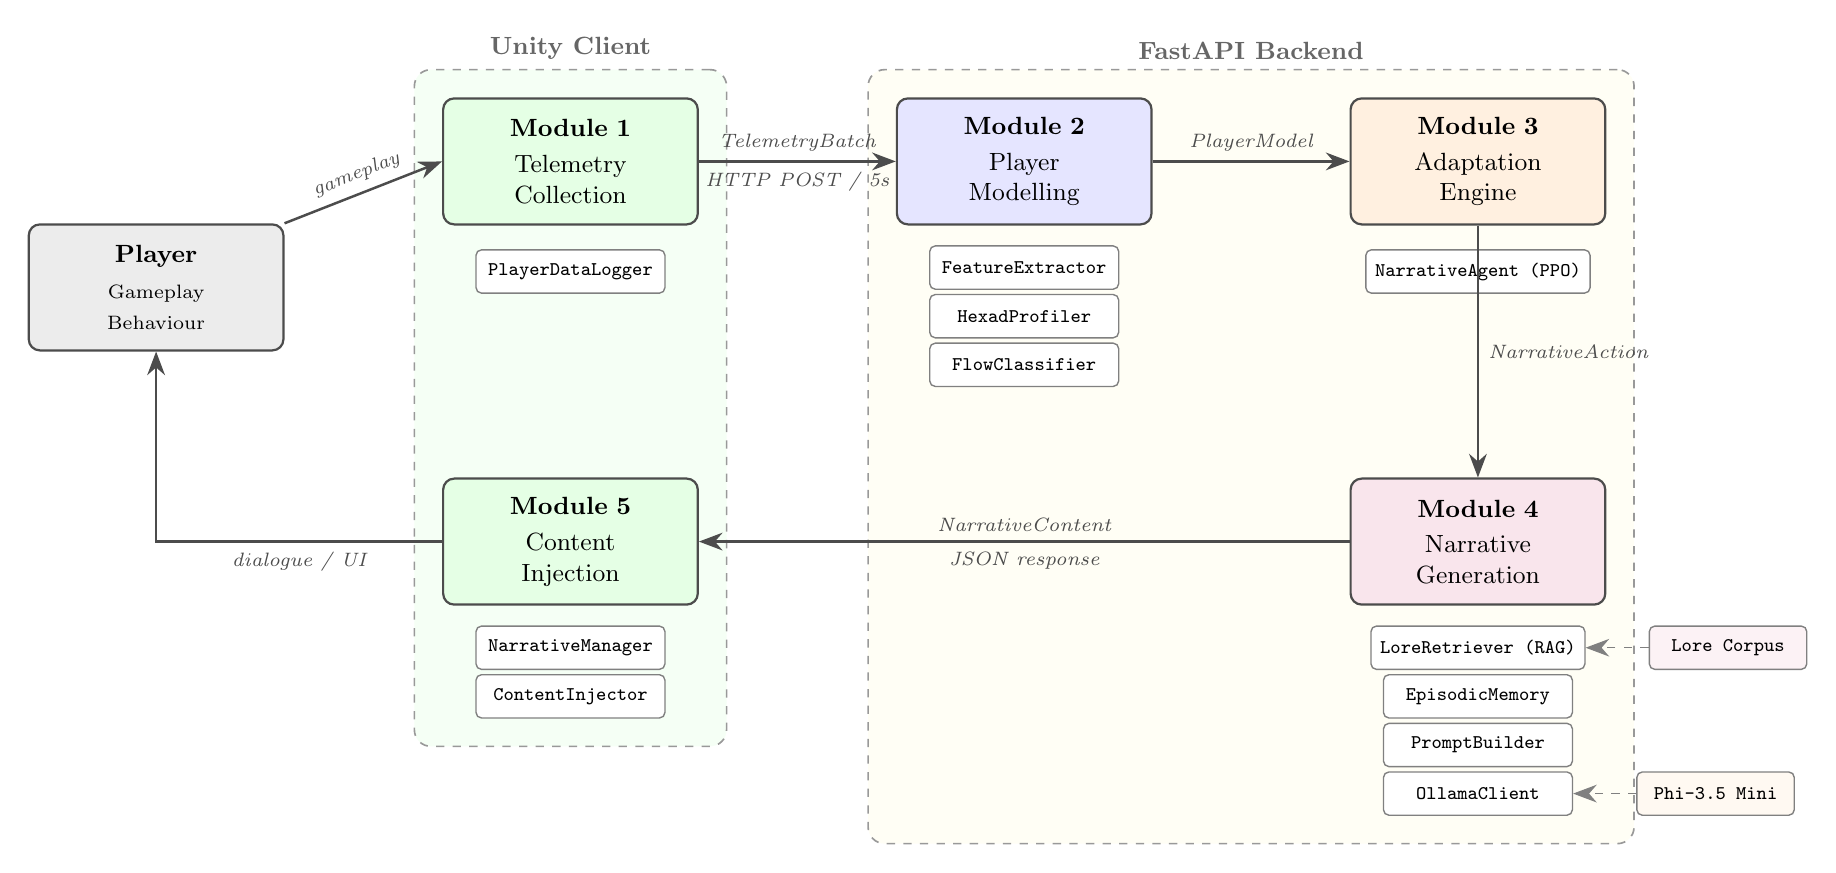
\begin{tikzpicture}[
    node distance=1.2cm and 1.8cm,
    >={Stealth[length=3mm]},
    module/.style={
        rectangle, rounded corners=4pt, draw=black!70, line width=0.8pt,
        fill=#1, minimum width=3.2cm, minimum height=1.6cm,
        text width=3cm, align=center, font=\small
    },
    module/.default={blue!8},
    component/.style={
        rectangle, rounded corners=2pt, draw=black!50, line width=0.5pt,
        fill=white, minimum width=2.4cm, minimum height=0.55cm,
        align=center, font=\scriptsize\ttfamily
    },
    data/.style={
        font=\scriptsize\itshape, text=black!70
    },
    arrow/.style={
        ->, line width=0.9pt, black!70
    },
    groupbox/.style={
        rectangle, rounded corners=6pt, draw=black!40, dashed,
        line width=0.6pt, inner sep=10pt
    }
]

% ── Module 1: Unity Client (Telemetry) ──
\node[module=green!10] (telemetry) {
    \textbf{Module 1}\\[2pt]
    Telemetry\\Collection
};
\node[component, below=0.3cm of telemetry] (pdl) {PlayerDataLogger};

% ── Module 2: Player Modelling ──
\node[module=blue!10, right=2.5cm of telemetry] (playermod) {
    \textbf{Module 2}\\[2pt]
    Player\\Modelling
};
\node[component, below=0.15cm of playermod, yshift=-0.1cm] (fe) {FeatureExtractor};
\node[component, below=0.05cm of fe] (hp) {HexadProfiler};
\node[component, below=0.05cm of hp] (fc) {FlowClassifier};

% ── Module 3: Adaptation Engine ──
\node[module=orange!12, right=2.5cm of playermod] (adaptation) {
    \textbf{Module 3}\\[2pt]
    Adaptation\\Engine
};
\node[component, below=0.3cm of adaptation] (ppo) {NarrativeAgent (PPO)};

% ── Module 4: Narrative Generation ──
\node[module=purple!10, below=3.2cm of adaptation] (narrative) {
    \textbf{Module 4}\\[2pt]
    Narrative\\Generation
};
\node[component, below=0.15cm of narrative, yshift=-0.1cm] (rag) {LoreRetriever (RAG)};
\node[component, below=0.05cm of rag] (mem) {EpisodicMemory};
\node[component, below=0.05cm of mem] (pb) {PromptBuilder};
\node[component, below=0.05cm of pb] (ollama) {OllamaClient};

% ── Module 5: Content Injection ──
\node[module=green!10, below=3.2cm of telemetry] (injection) {
    \textbf{Module 5}\\[2pt]
    Content\\Injection
};
\node[component, below=0.15cm of injection, yshift=-0.1cm] (nm) {NarrativeManager};
\node[component, below=0.05cm of nm] (ci) {ContentInjector};

% ── Player node ──
\node[module=gray!15, left=2.0cm of telemetry, yshift=-1.6cm] (player) {
    \textbf{Player}\\[2pt]
    {\scriptsize Gameplay}\\
    {\scriptsize Behaviour}
};

% ── Backend group box ──
\begin{scope}[on background layer]
    \node[groupbox, fill=yellow!4,
          fit=(playermod)(fe)(hp)(fc)(adaptation)(ppo)(narrative)(rag)(mem)(pb)(ollama),
          label={[font=\small\bfseries, text=black!60]above:FastAPI Backend}
    ] (backend) {};
\end{scope}

% ── Unity group box ──
\begin{scope}[on background layer]
    \node[groupbox, fill=green!4,
          fit=(telemetry)(pdl)(injection)(nm)(ci),
          label={[font=\small\bfseries, text=black!60]above:Unity Client}
    ] (unity) {};
\end{scope}

% ── Arrows ──
% Player -> Telemetry
\draw[arrow] (player.north east) -- node[data, above, sloped] {gameplay} (telemetry.west);

% Telemetry -> Player Modelling
\draw[arrow] (telemetry.east) -- node[data, above] {TelemetryBatch} node[data, below] {\scriptsize HTTP POST / 5s} (playermod.west);

% Player Modelling -> Adaptation
\draw[arrow] (playermod.east) -- node[data, above] {PlayerModel} (adaptation.west);

% Adaptation -> Narrative Generation
\draw[arrow] (adaptation.south) -- node[data, right, text width=2cm] {NarrativeAction} (narrative.north);

% Narrative Generation -> Content Injection
\draw[arrow] (narrative.west) -- node[data, above] {NarrativeContent} node[data, below] {\scriptsize JSON response} (injection.east);

% Content Injection -> Player
\draw[arrow] (injection.west) -| node[data, below, near start] {dialogue / UI} (player.south);

% ── Lore corpus annotation ──
\node[component, fill=purple!5, right=0.8cm of rag, minimum width=2cm] (lore) {Lore Corpus};
\draw[->, dashed, black!50] (lore) -- (rag);

% ── Ollama annotation ──
\node[component, fill=orange!5, right=0.8cm of ollama, minimum width=2cm] (phi) {Phi-3.5 Mini};
\draw[->, dashed, black!50] (phi) -- (ollama);

\end{tikzpicture}%
}
\caption{Closed-loop system architecture. Five modules form a pipeline from player behaviour through telemetry collection, player modelling, PPO-based adaptation, RAG-grounded narrative generation, and content injection back to the player. Dashed boxes indicate platform boundaries.}
\label{fig:architecture}
\end{figure}

The pipeline operates as a continuous loop, cycling once per telemetry window. The Unity \texttt{PlayerDataLogger} aggregates behavioural signals over five-second windows and transmits a \texttt{TelemetryBatch} to the FastAPI backend via HTTP POST (with WebSocket support available for lower-latency streaming when network conditions permit). On the backend, the Player Modelling Service processes each incoming batch through three sequential stages: the \texttt{FeatureExtractor} computes eleven normalised features from the raw telemetry, the \texttt{HexadProfiler} derives the six-dimensional continuous Hexad profile from the cumulative session history, and the \texttt{FlowClassifier} assigns a Flow state based on the most recent data. The assembled \texttt{PlayerModel} is then passed to the \texttt{NarrativeAgent}, which selects a \texttt{NarrativeAction} --- using the cold-start heuristic during the first 120~seconds, and the trained PPO policy thereafter. The Narrative Generation Service takes the selected action and uses it to formulate a query for the \texttt{LoreRetriever} (RAG), consults the \texttt{EpisodicMemory} for relevant prior narrative events, assembles the full two-message prompt through the \texttt{PromptBuilder}, and dispatches a generation request to the locally hosted Ollama LLM. The resulting \texttt{NarrativeContent} --- a JSON payload containing the generated text, content type, and speaker attribution --- is returned to the Unity client and injected at the appropriate in-game display point by the \texttt{ContentInjector}.

\section{Player Modelling Module}

The player modelling module is responsible for answering two questions about the player at every point in the session: \textit{what kind of player are they?} (the Hexad profile) and \textit{how are they doing right now?} (the Flow state). Everything downstream --- the action the PPO agent selects, the tone the LLM adopts, the content the player ultimately sees --- depends on the accuracy and responsiveness of these two answers.

\subsection{Telemetry Collection}

The telemetry system captures 23 behavioural fields per five-second window, providing the raw signal from which both the Hexad profile and the Flow state are derived. Table~\ref{tab:telemetry} lists the complete schema.

\begin{longtable}{@{}p{4cm} p{1.5cm} p{7.5cm}@{}}
\caption{TelemetryBatch schema (23 fields).} \label{tab:telemetry} \\
\toprule
\textbf{Field} & \textbf{Type} & \textbf{Description} \\
\midrule
\endfirsthead
\toprule
\textbf{Field} & \textbf{Type} & \textbf{Description} \\
\midrule
\endhead
player\_id & str & Unique player identifier \\
session\_id & str & Unique session identifier \\
window\_start & float & Window start time (Unix timestamp) \\
window\_end & float & Window end time (Unix timestamp) \\
kills & int & Enemy kills in window \\
deaths & int & Player deaths in window \\
damage\_taken & float & Total damage received \\
damage\_dealt & float & Total damage inflicted \\
abilities\_used & int & Ability activations \\
abilities\_hit & int & Abilities that connected \\
objectives\_completed & int & Objectives completed \\
objectives\_attempted & int & Objectives attempted \\
tiles\_explored & int & Map tiles visited \\
total\_tiles & int & Total traversable tiles (default 100) \\
npc\_interactions\_voluntary & int & Voluntary (unsolicited) NPC interactions \\
dialogue\_lines\_shown & int & Dialogue lines displayed \\
dialogue\_lines\_skipped & int & Dialogue lines skipped by player \\
lore\_items\_read & int & Lore collectibles read \\
lore\_items\_found & int & Lore collectibles discovered \\
idle\_seconds & float & Seconds with no player input \\
session\_elapsed & float & Total elapsed session time (seconds) \\
current\_location & str & Scene/zone identifier \\
current\_objective & str & Active quest objective identifier \\
\bottomrule
\end{longtable}

The five-second window granularity represents a deliberate trade-off between responsiveness and noise sensitivity. A shorter window would allow faster adaptation cycles but would amplify transient spikes --- a single unlucky death or a momentary pause to answer a phone call would distort the player model. A longer window would produce smoother signals but at the cost of delayed response: if a player tips from Flow into anxiety, the system should notice within seconds, not minutes. Five seconds proved to be a practical sweet spot during development. In practice, the system further smooths the signal by accumulating a sliding window of recent batches (typically six, spanning approximately 30~seconds) before computing the feature vector, allowing multi-window averages to absorb transient fluctuations.

\subsection{Feature Extraction (11 Features)}

The \texttt{FeatureExtractor} aggregates one or more \texttt{TelemetryBatch} records into eleven normalized scalar features, each clipped to [0, 1] (or [0, 3] for the \texttt{challenge\_skill\_ratio}). Table~\ref{tab:features} presents the computation formulae.

\begin{table}[H]
\centering
\caption{Eleven extracted features and computation formulae.}
\label{tab:features}
\small
\begin{tabular}{@{}p{3.5cm} p{6cm} p{3.5cm}@{}}
\toprule
\textbf{Feature} & \textbf{Formula} & \textbf{Notes} \\
\midrule
kd\_ratio & clip(kills / max(deaths, 1) / 5.0, 0, 1) & Norm.\ at 5:1 K/D \\
objective\_rate & clip(obj\_comp / max(obj\_att, 1), 0, 1) & Completion proportion \\
explore\_rate & clip(tiles\_explored / total\_tiles, 0, 1) & Map coverage \\
dialogue\_engage & clip(1 $-$ skipped / max(shown, 1), 0, 1) & 1 = reads all \\
ability\_accuracy & clip(hit / max(used, 1), 0, 1) & Combat precision \\
damage\_taken\_norm & clip(dmg / (elapsed\_min + 1) / 200, 0, 1) & DPM normalized \\
idle\_ratio & clip(idle\_s / elapsed, 0, 1) & Fraction idle \\
lore\_engage\_rate & clip(read / max(found, 1), 0, 1) & Lore depth \\
skill\_score & 0.35 kd + 0.30 obj + 0.20 acc + 0.15(1$-$idle) & Composite skill \\
challenge\_score & 0.50 dmg + 0.30(1$-$obj) + 0.20 death\_ratio & Composite challenge \\
challenge\_skill\_ratio & clip(challenge / max(skill, $10^{-6}$), 0, 3) & Core Flow signal \\
\bottomrule
\end{tabular}
\end{table}

The \texttt{skill\_score} composite weights combat effectiveness (\texttt{kd\_ratio}, \texttt{ability\_accuracy}) most heavily, followed by objective completion and attention (inverse \texttt{idle\_ratio}). The \texttt{challenge\_score} composite weights damage pressure most heavily, followed by objective failure rate and death rate. Dividing challenge by skill yields the \texttt{challenge\_skill\_ratio}, which operationalizes Csikszentmihalyi's (\citeyear{csikszentmihalyi1990flow}) challenge--skill balance axis.

\subsection{Hexad Profile Computation (6 Dimensions)}

The \texttt{HexadProfiler} computes six continuous scores in [0, 1] from accumulated telemetry, each representing the strength of a Hexad player-type signal. Table~\ref{tab:hexad} shows the computation weights.

\begin{table}[H]
\centering
\caption{Hexad dimension computation weights from telemetry signals.}
\label{tab:hexad}
\small
\begin{tabular}{@{}p{2.5cm} p{7cm} p{3.5cm}@{}}
\toprule
\textbf{Dimension} & \textbf{Formula} & \textbf{Interpretation} \\
\midrule
Achiever & 0.70 $\times$ obj\_rate + 0.30 $\times$ norm(kills, 20) & Objective + combat \\
Explorer & 0.50 $\times$ explore\_rate + 0.50 $\times$ lore\_rate & Map + lore coverage \\
Socializer & 0.60 $\times$ norm(vol\_npc, 10) + 0.40 $\times$ dialogue & Seeks NPCs + reads \\
Free Spirit & 0.50 $\times$ explore\_rate + 0.50 $\times$ (1 $-$ obj\_rate) & Explores off-path \\
Disruptor & 0.65 $\times$ norm(kills, 20) + 0.15 $\times$ norm(deaths, 10) + 0.20 $\times$ norm(dmg, 1000) & Aggressive combat \\
Philanthropist & 0.60 $\times$ dialogue\_engage + 0.40 $\times$ lore\_rate & Narrative engagement \\
\bottomrule
\end{tabular}
\end{table}

The mapping from behavioural signals to Hexad dimensions was established through a principled alignment process guided by the original Hexad motivation descriptions \citep{tondello2016hexad}. The logic proceeds dimension by dimension. Achievers seek mastery and progress, so the signal proxies are objective completion rate and combat kill count --- both direct indicators of goal-oriented play. Explorers seek discovery, so map coverage and lore engagement serve as proxies: a player who visits every corner of the map and reads every collectible is behaving as an Explorer regardless of what a questionnaire might say. Socializers seek connection, so voluntary NPC interaction count and dialogue engagement rate are weighted; a player who seeks out NPCs unprompted and reads their dialogue is exhibiting Socializer behaviour. Free Spirits resist imposed structure, so the proxy is exploration \textit{uncorrelated with} objective completion --- wandering off the critical path rather than following it. Disruptors challenge systems, captured by aggressive combat behaviour (high kill counts, high damage dealt, willingness to die repeatedly). Philanthropists give and share, captured by depth of engagement with narrative and lore content --- a proxy for the motivation to understand and connect with the game world rather than merely to conquer it.

All profiles are initialised to 0.5 (the neutral midpoint) in the absence of data, preventing cold-start artefacts from biasing the narrative action selection before the system has observed enough behaviour to form a meaningful profile.

\subsection{Flow State Classification (MDP States)}

The \texttt{FlowClassifier} implements a decision-tree classifier over the \texttt{challenge\_skill\_ratio}, \texttt{idle\_ratio}, and \texttt{dialogue\_engage\_rate} features. Table~\ref{tab:flow_rules} formalizes the rules.

\begin{table}[H]
\centering
\caption{Flow state classification rules (evaluated in priority order).}
\label{tab:flow_rules}
\small
\begin{tabular}{@{}clll@{}}
\toprule
\textbf{Priority} & \textbf{Condition} & \textbf{State} & \textbf{Confidence} \\
\midrule
1 (highest) & idle $>$ 0.40 AND dialogue $<$ 0.30 AND ratio $<$ 0.60 & APATHY & 0.70 \\
2 & ratio $<$ 0.75 & BOREDOM & 0.60 + (0.75 $-$ ratio) $\times$ 0.80 \\
3 & ratio $>$ 1.30 & ANXIETY & 0.60 + (ratio $-$ 1.30) $\times$ 0.40 \\
4 (default) & 0.75 $\leq$ ratio $\leq$ 1.30 & FLOW & max(0.55, 1.0 $-$ $|$ratio $-$ 1.0$|$ $\times$ 1.2) \\
\bottomrule
\end{tabular}
\end{table}

Figure~\ref{fig:flow_tree} visualises the classification logic as a decision tree.

\begin{figure}[H]
\centering
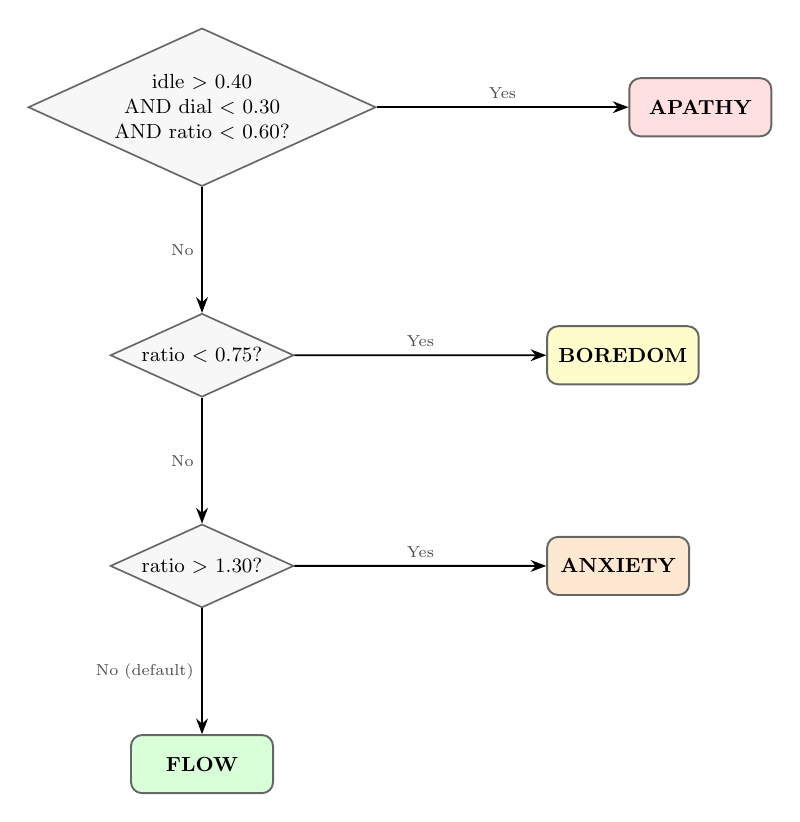
\begin{tikzpicture}[
    scale=0.82, every node/.style={scale=0.82},
    >={Stealth[length=2mm]},
    decision/.style={
        diamond, draw=black!60, line width=0.6pt, fill=gray!6,
        inner sep=2pt, align=center, font=\small,
        minimum width=2.2cm, aspect=2.2
    },
    outcome/.style={
        rectangle, rounded corners=4pt, draw=black!60, line width=0.7pt,
        minimum width=2.2cm, minimum height=0.9cm,
        align=center, font=\small\bfseries, inner sep=5pt
    },
    edgelbl/.style={font=\scriptsize, text=black!70},
]

% ── Decision nodes ──
\node[decision] (d1) {idle $>$ 0.40\\AND dial $<$ 0.30\\AND ratio $<$ 0.60?};
\node[outcome, fill=red!12, right=3.2cm of d1] (apathy) {APATHY};

\node[decision, below=1.6cm of d1] (d2) {ratio $<$ 0.75?};
\node[outcome, fill=yellow!20, right=3.2cm of d2] (boredom) {BOREDOM};

\node[decision, below=1.6cm of d2] (d3) {ratio $>$ 1.30?};
\node[outcome, fill=orange!18, right=3.2cm of d3] (anxiety) {ANXIETY};

\node[outcome, fill=green!15, below=1.6cm of d3] (flow) {FLOW};

% ── Edges ──
\draw[->, line width=0.7pt] (d1) -- node[edgelbl, above] {Yes} (apathy);
\draw[->, line width=0.7pt] (d1) -- node[edgelbl, left] {No} (d2);
\draw[->, line width=0.7pt] (d2) -- node[edgelbl, above] {Yes} (boredom);
\draw[->, line width=0.7pt] (d2) -- node[edgelbl, left] {No} (d3);
\draw[->, line width=0.7pt] (d3) -- node[edgelbl, above] {Yes} (anxiety);
\draw[->, line width=0.7pt] (d3) -- node[edgelbl, left] {No (default)} (flow);

\end{tikzpicture}
\caption{Flow state classification decision tree. Conditions are evaluated in priority order (top to bottom); the first satisfied condition determines the classification.}
\label{fig:flow_tree}
\end{figure}

The priority ordering matters. APATHY is evaluated first because it represents a qualitatively distinct disengagement pattern --- the player has not merely lost interest in the challenge (which would be BOREDOM) but has stopped meaningfully interacting with the game altogether. Without the compound condition check, such a player would be classified as BORED on the challenge--skill ratio alone, and the system would respond with urgency-boosting narrative. But a disengaged player does not need urgency; they need a reason to care. The APATHY classification ensures the system responds with mystery and intrigue rather than pressure.

The confidence scoring for BOREDOM and ANXIETY is proportional to the distance from the FLOW band boundary: a player with a challenge--skill ratio of 0.40 is classified with higher confidence than one at 0.70, because the former is further from the zone of optimal engagement. FLOW confidence is highest when the ratio sits closest to 1.0 --- the theoretical point of perfect challenge--skill balance --- and tapers as the ratio approaches either boundary.

\section{Narrative Generation Module}

The narrative generation module is the part of the system that actually writes the story. Everything upstream --- the telemetry, the feature extraction, the Flow classification, the Hexad profiling, the PPO action selection --- exists to inform this module about \textit{what kind of narrative to produce}. The module itself is responsible for producing it: grounded in the game's lore, consistent with the session's narrative history, and formatted for injection into the game's UI.

\subsection{RAG Pipeline}

The \texttt{LoreRetriever} implements in-memory semantic search using the sentence-transformers all-MiniLM-L6-v2 model, which produces 384-dimensional L2-normalised embeddings. The lore corpus --- comprising the world, character, and quest lore documents stored in the \texttt{lore/} directory --- is pre-indexed at server startup. Each document is chunked by paragraph (double-newline delimiters), and each chunk is embedded into the 384-dimensional space. At retrieval time, the query (constructed from the player's current Flow state, activity, and location) is embedded and cosine similarities are computed against all stored chunk embeddings via a dot product (since all vectors are unit-normalised, cosine similarity reduces to the dot product). The top $k = 3$ chunks by similarity are returned and formatted as bullet points in the LLM user prompt, providing the model with the lore context most relevant to the current generation task.

This design was chosen over a persistent vector database (e.g., ChromaDB, Pinecone) for two reasons that proved decisive during development. First, ChromaDB's Pydantic v1 dependency created compatibility issues with the project's Python 3.14 runtime that could not be cleanly resolved. Second, and more fundamentally, the lore corpus is small --- three files, approximately 30 paragraphs, a few hundred embeddings at most --- which renders the indexing, persistence, and query optimisation machinery of a full vector database unnecessary overhead. In-memory retrieval at this corpus scale completes in sub-millisecond time, well within the latency budget of the narrative generation pipeline.

\subsection{Episodic Session Memory}

The \texttt{EpisodicMemory} class maintains a capped list of \texttt{MemoryEvent} records, each comprising a text description, an importance score in [0, 1], and a timestamp. When the list exceeds the maximum capacity of ten events, it is sorted by importance in descending order and truncated to the top ten. This importance-weighted eviction ensures that the most narratively significant events are retained even as minor events accumulate.

At prompt construction time, the top five events by importance score are selected and formatted as a context block, providing the LLM with a compressed narrative history that enables references to past events and prevents temporal inconsistency.

\subsection{Dynamic Prompt Construction}

The \texttt{PromptBuilder} assembles a two-message prompt (system + user) for the Ollama API. The system prompt encodes the LLM's role (narrative writer for the game world), output length constraints (2--4 sentences for dialogue, 1--2 for descriptions), format requirements (valid JSON only, specific schema), and the emotional tone mapped from the current Flow state:

\begin{itemize}
\item ANXIETY: ``urgent and supportive --- the player is struggling''
\item BOREDOM: ``exciting and surprising --- inject energy''
\item FLOW: ``immersive and atmospheric --- maintain the experience''
\item APATHY: ``intriguing and mysterious --- re-engage the player''
\end{itemize}

The user prompt injects: the player's current Flow state and challenge--skill ratio; the current activity (IN\_COMBAT, EXPLORING, IN\_DIALOGUE, IDLE); session elapsed time; the Hexad profile percentages; the selected NarrativeAction with definitions; the current location and active quest stage; the three retrieved lore chunks; the episodic memory context; and explicit content constraints (no real-world references, no anachronisms, no fourth-wall breaks, character voice descriptions).

\subsection{LLM Integration (Ollama / Phi-3.5 Mini)}

The \texttt{OllamaClient} sends the assembled prompt to a locally hosted Ollama instance using the \texttt{/api/chat} endpoint. The primary model is Phi-3.5 Mini (3.8B parameters; \citealp{microsoft2024phi}), with Llama 3.2 3B as a configured fallback. The generation parameters are: temperature 0.75, top\_p 0.90, maximum tokens 200, JSON format mode enabled. The 8-second HTTP timeout ensures that a slow or stalled generation does not block the main game loop.

When the LLM response is malformed JSON, contains a fallback signal, or the request times out, the \texttt{OllamaClient} returns a pre-authored fallback string corresponding to the requested \texttt{NarrativeAction}. These fallback strings are intentionally minimal --- a single sentence of tonally appropriate narrative --- designed to maintain the illusion of a functioning narrative system without exposing the player to error messages, empty dialogue boxes, or other artefacts that would break immersion. The player sees a brief, contextually appropriate line; they do not see that the LLM failed to produce valid output. This graceful degradation is essential for a system that will be used in a controlled user study, where a single visible error could contaminate a participant's experience and compromise the evaluation.

\section{Adaptation Engine (MDP + PPO)}

The adaptation engine is the decision-making core of the system: given what the player modelling module knows about the player right now, what should the narrative do next? This question is formalised as a reinforcement learning problem, which allows the answer to be \textit{learned} from experience rather than hand-coded by the designer.

\subsection{MDP Formulation}

The narrative adaptation problem is formalised as a Markov Decision Process $(S, A, T, R, \gamma)$ implemented as a Gymnasium environment.

\textbf{State space $S$:} A Box observation space of shape (7,) with all values in [0, 1]. Table~\ref{tab:mdp_state} defines the seven dimensions.

\begin{table}[H]
\centering
\caption{MDP observation vector (7 dimensions).}
\label{tab:mdp_state}
\small
\begin{tabular}{@{}clp{7cm}@{}}
\toprule
\textbf{Index} & \textbf{Signal} & \textbf{Description} \\
\midrule
0 & flow\_score & Encoded Flow state (FLOW=1.0, BOREDOM=0.3, ANXIETY=0.2, APATHY=0.1) \\
1 & csr\_norm & challenge\_skill\_ratio / 3.0 \\
2 & hexad\_explorer & Explorer dimension score \\
3 & hexad\_socializer & Socializer dimension score \\
4 & hexad\_achiever & Achiever dimension score \\
5 & hexad\_disruptor & Disruptor dimension score \\
6 & session\_progress & session\_elapsed / 1800.0 (normalized to 30-min max) \\
\bottomrule
\end{tabular}
\end{table}

\textbf{Action space $A$:} A Discrete(8) action space corresponding to the eight \texttt{NarrativeAction} values. Table~\ref{tab:actions} summarizes the actions.

\begin{table}[H]
\centering
\caption{Eight narrative actions with descriptions and intended effects.}
\label{tab:actions}
\small
\begin{tabular}{@{}cll@{}}
\toprule
\textbf{Idx} & \textbf{Action} & \textbf{Intended Effect} \\
\midrule
0 & LOWER\_STAKES & Reduce narrative tension; provide respite \\
1 & RAISE\_STAKES & Increase narrative urgency and weight \\
2 & ADD\_MYSTERY & Introduce a curiosity hook or unexplained element \\
3 & ADD\_HUMOR & Provide comic relief to reduce tension \\
4 & PROVIDE\_GUIDANCE & Give struggling player directional narrative support \\
5 & INCREASE\_URGENCY & Re-energize a bored or disengaged player \\
6 & LORE\_REWARD & Deliver a lore discovery payoff for curious players \\
7 & NO\_CHANGE & Suppress narrative injection; maintain current experience \\
\bottomrule
\end{tabular}
\end{table}

\textbf{Transition dynamics $T$:} The simulated training environment models stochastic Flow state transitions. When the agent selects a ``helpful'' action for the current state (e.g., ANXIETY $\rightarrow$ \{PROVIDE\_GUIDANCE, LOWER\_STAKES\}), the environment transitions to FLOW with probability 0.75 or remains in the current state with probability 0.25. This stochasticity prevents the policy from memorizing a deterministic mapping and encourages generalization across states.

Figure~\ref{fig:mdp_transitions} visualises the state transitions and the narrative actions that drive them.

\begin{figure}[H]
\centering
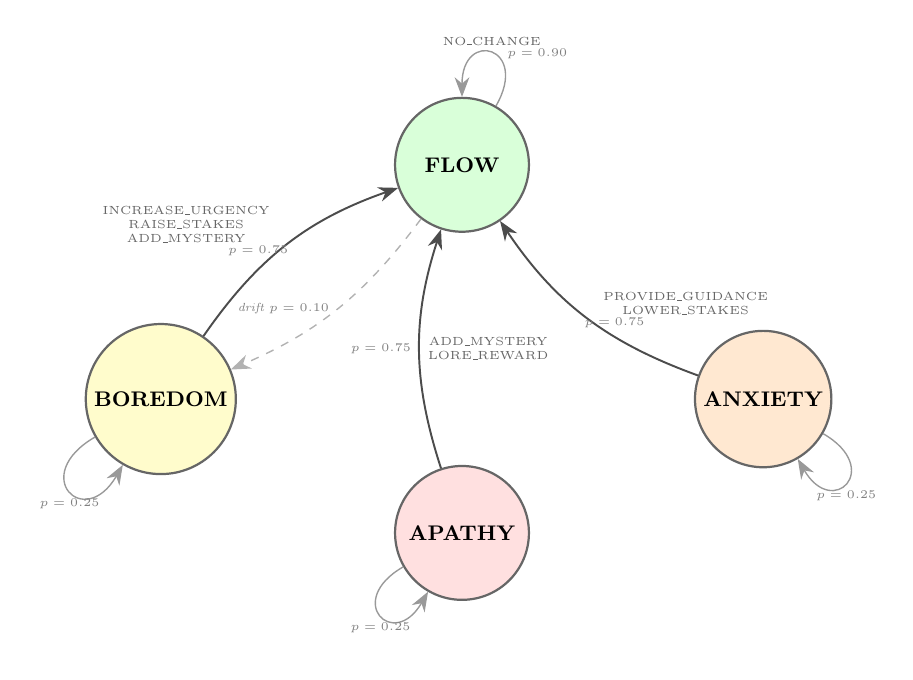
\begin{tikzpicture}[
    scale=0.85, every node/.style={scale=0.85},
    >={Stealth[length=2.5mm]},
    state/.style={
        circle, draw=black!60, line width=0.8pt,
        minimum size=2cm, align=center, font=\small\bfseries, inner sep=3pt
    },
    helpful/.style={->, line width=0.7pt, black!70, bend left=18},
    selfloop/.style={->, line width=0.5pt, black!40, looseness=5},
    drift/.style={->, line width=0.5pt, black!30, dashed, bend left=15},
    actlbl/.style={font=\tiny, text=black!60, align=center},
    problbl/.style={font=\tiny\itshape, text=black!50},
]

% ── States ──
\node[state, fill=green!15] (flow)    at (0,0)      {FLOW};
\node[state, fill=yellow!20] (bore)   at (-4.5,-3.5) {BOREDOM};
\node[state, fill=orange!18] (anx)    at (4.5,-3.5)  {ANXIETY};
\node[state, fill=red!12]   (apa)     at (0,-5.5)    {APATHY};

% ── Helpful actions → FLOW (p=0.75) ──
\draw[helpful] (bore) to
    node[actlbl, above left, pos=0.45] {INCREASE\_URGENCY\\RAISE\_STAKES\\ADD\_MYSTERY}
    node[problbl, below left, pos=0.55] {$p=0.75$}
    (flow);
\draw[helpful] (anx) to
    node[actlbl, above right, pos=0.45] {PROVIDE\_GUIDANCE\\LOWER\_STAKES}
    node[problbl, below right, pos=0.55] {$p=0.75$}
    (flow);
\draw[helpful] (apa) to
    node[actlbl, right, pos=0.5] {ADD\_MYSTERY\\LORE\_REWARD}
    node[problbl, left, pos=0.5] {$p=0.75$}
    (flow);

% ── Self-loops (remain, p=0.25 or unhelpful) ──
\draw[selfloop] (bore) to[out=210, in=240] node[problbl, below] {$p=0.25$} (bore);
\draw[selfloop] (anx) to[out=-30, in=-60] node[problbl, below] {$p=0.25$} (anx);
\draw[selfloop] (apa) to[out=210, in=240] node[problbl, below] {$p=0.25$} (apa);

% ── FLOW self-loop (NO_CHANGE) ──
\draw[selfloop] (flow) to[out=60, in=90]
    node[actlbl, above] {NO\_CHANGE}
    node[problbl, right, xshift=3pt] {$p=0.90$}
    (flow);

% ── Drift from FLOW → BOREDOM ──
\draw[drift] (flow) to
    node[problbl, left, pos=0.5] {drift $p=0.10$}
    (bore);

\end{tikzpicture}
\caption{MDP state-transition diagram. Solid arrows show transitions caused by helpful narrative actions ($p = 0.75$ to FLOW). Self-loops indicate remaining in the current state. The dashed arrow shows the stochastic drift from FLOW to BOREDOM when no helpful action is needed.}
\label{fig:mdp_transitions}
\end{figure}

\textbf{Discount factor $\gamma$:} 0.95, reflecting moderate preference for near-term reward while maintaining long-horizon planning.

\subsection{Reward Function Design}

The reward function is defined over (prev\_state, new\_state, action, steps\_in\_state, last\_3\_actions) and comprises five components, detailed in Table~\ref{tab:reward}.

\begin{table}[H]
\centering
\caption{Reward function components and values.}
\label{tab:reward}
\small
\begin{tabular}{@{}lll@{}}
\toprule
\textbf{Component} & \textbf{Value} & \textbf{Trigger} \\
\midrule
State reward (FLOW) & $+1.0$ & new\_state == FLOW \\
State reward (BOREDOM) & $-0.3$ & new\_state == BOREDOM \\
State reward (ANXIETY) & $-0.5$ & new\_state == ANXIETY \\
State reward (APATHY) & $-0.8$ & new\_state == APATHY \\
Step penalty & $-0.05$ & Every step \\
Flow streak bonus & $+0.20$ & FLOW AND steps\_in\_state $>$ 2 \\
Transition bonus & $+0.30$ & prev $\in$ \{ANXIETY, BOREDOM\} AND new == FLOW \\
Repetition penalty & $-0.15$ & All 3 recent actions identical \\
\bottomrule
\end{tabular}
\end{table}

The reward function encodes a clear priority ordering. APATHY draws the heaviest penalty ($-0.8$) because it represents the deepest disengagement --- a player who has essentially given up. ANXIETY ($-0.5$) is penalised more than BOREDOM ($-0.3$) because an overwhelmed player is at higher risk of quitting the session entirely. The step penalty ($-0.05$) applies at every timestep regardless of state, creating constant pressure toward action efficiency and discouraging the agent from drifting into passive NO\_CHANGE loops. The Flow streak bonus ($+0.20$) rewards sustained optimal experience, not just momentary hits of Flow: it activates only after the player has been in FLOW for more than two consecutive steps, encouraging the agent to maintain conditions rather than simply reaching them. The transition bonus ($+0.30$) provides additional shaping reward for the key recovery transitions --- moving a player from ANXIETY or BOREDOM back into FLOW --- which are the most valuable moments for the system to get right. Finally, the repetition penalty ($-0.15$) fires when all three most recent actions are identical, discouraging degenerate policies in which the agent converges on a single favourite action and applies it regardless of context.

\subsection{Cold-Start Heuristic}

For the first 120~seconds of a session, or when the PPO model is unavailable, the \texttt{NarrativeAgent} falls back to a deterministic heuristic policy:

\begin{itemize}
\item ANXIETY $\rightarrow$ PROVIDE\_GUIDANCE
\item BOREDOM $\rightarrow$ INCREASE\_URGENCY
\item APATHY $\rightarrow$ ADD\_MYSTERY
\item FLOW $\rightarrow$ NO\_CHANGE
\end{itemize}

The 120-second threshold serves a dual purpose. It gives the player time to settle into the game world --- learning the controls, orienting to the environment, forming initial goals --- before the learned policy begins making adaptation decisions. And it gives the player modelling module time to accumulate enough telemetry for the Hexad profile and Flow classification to be meaningful. A PPO policy operating on a player model derived from ten seconds of data would be making decisions on noise; the heuristic ensures that the first two minutes of narrative adaptation are sensible even when the signal is thin.

\section{Unity Plugin Design}

The Unity plugin comprises three C\# components: \texttt{PlayerDataLogger}, \texttt{NarrativeManager}, and \texttt{ContentInjector}.

\texttt{PlayerDataLogger} is a MonoBehaviour that maintains running accumulators for all 23 telemetry fields. Every five seconds, it serializes the accumulated values into a \texttt{TelemetryBatch} JSON object and dispatches it to the FastAPI backend via an async HTTP POST. It exposes a public API for game systems to register events: \texttt{RecordKill()}, \texttt{RecordDeath()}, \texttt{RecordDialogueShown()}, and others. This event-based registration model decouples the telemetry system from specific game mechanics, making the plugin applicable to any Unity game that exposes these event hooks.

\texttt{NarrativeManager} polls the \texttt{/narrative/generate} endpoint following each telemetry transmission. \texttt{ContentInjector} maps \texttt{NarrativeContentType} to the appropriate UI mechanism: dialogue content is routed to the DialoguePanel, description content to the DescriptionPanel, and quest updates to the QuestLog. The injector implements a content queue with a 3-second minimum spacing between consecutive injections to prevent narrative overcrowding.

For the Control condition, the \texttt{NarrativeManager} is replaced by a \texttt{StaticNarrativeManager} that reads from a \texttt{StaticNarrativeContent} ScriptableObject and fires narrative events at scripted triggers with no player-state dependency.

\section{Testbed Game Design}

The testbed is a 3D RPG built in Unity 6 LTS using the AnyRPG Core framework \citep{anyrpg2024core}. AnyRPG provides a complete RPG engine --- combat, questing, inventory, NPC dialogue, and character progression --- out of the box, which allowed the development effort to focus on the narrative personalization system rather than on reimplementing standard RPG mechanics from scratch.

The game world is set in the Contested Vale, a once-fertile trade corridor now fought over by two rival factions. The setting was chosen to support a range of player behaviours: combat encounters for Achievers and Disruptors, exploration opportunities for Explorers and Free Spirits, NPC interactions for Socializers, and lore collectibles for Philanthropists. The world is described in structured lore documents (stored in the \texttt{lore/} directory) that double as the RAG corpus for the narrative generation pipeline.

Three navigable areas make up the game world:

\begin{enumerate}
\item \textbf{Commander Varis's Post} --- a fortified camp at the northern edge serving as the starting area. Varis is the primary quest giver: a methodical, unsentimental military commander who gives orders without explaining them. Players who engage extensively with Varis register high Achiever signals.

\item \textbf{The Contested Zone} --- a combat-focused area containing enemy units and environmental hazards. Players who clear this area efficiently register high Achiever and Disruptor signals; players who explore its periphery register Explorer signals.

\item \textbf{The Waystone / Chronicler's Camp} --- a neutral area where the Chronicler, a scholar who has observed the Vale for thirty years, provides lore and context. The presence of lore collectibles creates a natural Explorer/Philanthropist signal divergence.
\end{enumerate}

Three NPCs populate the world, each designed with a distinct voice and function that the LLM must maintain when generating dialogue for them. Commander Varis is the primary quest giver: a methodical, unsentimental military officer who gives orders and expects compliance. The Chronicler is the lore source: a scholar who has observed the Vale for thirty years and speaks in measured, academic prose. Sera the Merchant is the pragmatic intermediary: a supply trader whose dialogue is clipped, transactional, and occasionally sardonic. These three voices serve as a consistency test for the narrative generation pipeline --- if the LLM generates dialogue for the Chronicler that sounds like Varis, the player will notice.

The main quest (Clear the Advance) provides a linear spine through the combat zone, ensuring that all players encounter a minimum threshold of challenge and narrative content. A secondary collection quest (Salvage the Fallen) encourages off-path exploration and rewards lore engagement. A standard play session runs approximately 25--30 minutes, which is long enough for the player modelling module to build a meaningful profile but short enough to remain practical within the constraints of a controlled user study.

\section{Evaluation Design}

\subsection{Research Hypotheses}

The following directional hypotheses are tested:

\begin{description}
\item[H1:] Participants in the Experimental condition will score significantly higher on the GEQ Flow subscale than participants in the Control condition.
\item[H2:] Participants in the Experimental condition will score significantly higher on the GEQ Immersion subscale than participants in the Control condition.
\item[H3:] Participants in the Experimental condition will score significantly higher on the NPS-3 Narrative Personalization Scale than participants in the Control condition.
\end{description}

H1 is designated the primary hypothesis because Flow is the direct optimisation target of the adaptation engine's reward function. If the system works as designed, H1 is the hypothesis it is most likely to support; if the system fails, H1 is the hypothesis that will be most clearly refuted.

\subsection{Participants and Recruitment}

A total of $N = 50$ participants are recruited (25 Experimental, 25 Control) via convenience sampling through university mailing lists and gaming society channels. Inclusion criteria: aged 18 or over; self-reported experience playing RPG or action-adventure games; no prior exposure to the testbed game. An a priori power analysis for Welch's independent-samples $t$-test targeting $d = 0.5$ (medium effect), $\alpha = 0.05$ (two-tailed), and $1 - \beta = 0.80$ yields a required sample size of approximately 51 total participants \citep{faul2007gpower}, indicating that $N = 50$ is marginally below the strict threshold but remains reasonable given practical constraints.

Participants are randomly assigned to conditions using a balanced random allocation procedure. No block randomization by demographic is applied, given the expected homogeneity of the university convenience sample.

\subsection{Instruments}

\textbf{Game Experience Questionnaire (GEQ) --- Core Module.} The GEQ \citep{ijsselsteijn2013geq} is a 33-item instrument measuring seven dimensions of game experience on a 0--4 scale. The primary DV is the GEQ \textbf{Flow subscale} (items 5, 13, 25, 28, 31; items 5 and 13 reverse-scored). The secondary DV is the GEQ \textbf{Immersion subscale} (items 3, 12, 18, 19, 27, 30).

\textbf{miniPXI --- Player Experience Inventory (Short Form).} The miniPXI \citep{vornhagen2022minipxi} is an 11-item instrument on a 1--7 scale covering six player experience dimensions. The total score (mean of all 11 items) is used as a general player experience index.

\textbf{Narrative Personalization Scale (NPS-3).} The NPS-3 is a custom three-item scale on a 1--7 Likert scale: (1) ``The story felt tailored to how I was playing,'' (2) ``The narrative responded to my choices and actions,'' and (3) ``The game seemed to understand what kind of player I am.'' Cronbach's alpha will be reported; if $\alpha < 0.70$, items will be analysed individually.

\textbf{Behavioural Metrics (from telemetry).} Three behavioural metrics derived from telemetry serve as objective secondary measures: voluntary NPC interactions, dialogue read ratio, and exploration coverage.

\subsection{Procedure}

Each participant session follows a standardized procedure conducted individually:

\begin{enumerate}
\item \textbf{Arrival and consent} (5 min): briefing, participant information sheet, informed consent, audio recording consent.
\item \textbf{Tutorial} (5 min): condition-identical tutorial scene familiarizing participants with movement, combat, and NPC interaction.
\item \textbf{Game session} (25--30 min): participant plays in their assigned condition. The researcher is present but silent. Session is time-limited to 30 minutes.
\item \textbf{Questionnaires} (10 min): GEQ Core Module, miniPXI, and NPS-3 completed immediately post-session.
\item \textbf{Semi-structured interview} (20 min): following the interview guide (Appendix~\ref{app:interview}), audio recorded.
\item \textbf{Debrief} (5 min): explanation of the system and opportunity for questions.
\end{enumerate}

Total session duration: approximately 65 minutes per participant.

\subsection{Ethical Considerations}

This research received ethical approval through the institutional SPER process. All participants provide informed consent prior to participation and are informed of their right to withdraw at any time without penalty. Telemetry data is stored locally on the research machine in a SQLite database without personally identifiable information beyond the session identifier. Audio recordings from interviews are stored on an encrypted drive and transcribed with participant consent. All data is handled in accordance with GDPR requirements and university data protection policy. Participants are debriefed following the session and informed of the study's full purpose.

\subsection{Analysis Plan}

\textbf{Quantitative analysis} follows these steps:

\begin{enumerate}
\item \textbf{Normality assessment:} Shapiro-Wilk tests per DV per condition. If normality is violated ($p < 0.05$), Mann-Whitney U is substituted for Welch's $t$-test.
\item \textbf{Primary test (H1):} Welch's independent-samples $t$-test comparing GEQ Flow subscale scores. Effect size reported as Cohen's $d$ \citep{cohen1988statistical}.
\item \textbf{Secondary tests (H2, H3):} Identical procedure. Bonferroni correction applied across three hypotheses ($\alpha_{\text{adj}} = 0.0167$).
\item \textbf{Reliability:} Cronbach's alpha computed for each subscale.
\item \textbf{Behavioural metrics:} Welch's $t$-tests as exploratory analyses without correction.
\end{enumerate}

\textbf{Qualitative analysis} follows the six-phase Reflexive Thematic Analysis procedure \citep{braun2022thematic}: familiarization, coding, constructing themes, reviewing, defining themes, and writing up with representative quotes.

%##########################################################################
% CHAPTER 4: RESULTS
%##########################################################################
\chapter{Results}

\section{Chapter Overview}

This chapter presents the findings of the between-subjects user study. The quantitative results are reported first (demographics, hypothesis tests, behavioural metrics), followed by the qualitative themes derived from semi-structured interviews via Reflexive Thematic Analysis. All statistical analyses were conducted using the procedures specified in Section~3.9.

\section{Participant Demographics}

A total of $N = 50$ participants completed the study. One participant in the Control condition was excluded due to a technical failure (the backend server crashed at the 8-minute mark, resulting in incomplete telemetry), yielding a final sample of $N = 49$ (25 Experimental, 24 Control). Table~\ref{tab:demographics} summarizes the demographic characteristics of the sample.

\begin{table}[H]
\centering
\caption{Participant demographics.}
\label{tab:demographics}
\small
\begin{tabular}{@{}llll@{}}
\toprule
\textbf{Variable} & \textbf{Exp.\ ($n$=25)} & \textbf{Ctrl.\ ($n$=24)} & \textbf{Total ($N$=49)} \\
\midrule
Age: Mean (SD) & 22.4 (2.1) & 21.9 (2.3) & 22.2 (2.2) \\
Gender: F / M & 9 / 16 & 8 / 16 & 17 / 32 \\
Gaming hours/week: Mean (SD) & 12.8 (6.4) & 13.5 (7.1) & 13.1 (6.7) \\
RPG experience (1--5): Mean (SD) & 3.6 (0.9) & 3.4 (1.0) & 3.5 (1.0) \\
\bottomrule
\end{tabular}
\end{table}

No significant baseline differences between conditions were observed on age ($t$(47) = 0.81, $p$ = .42) or gaming hours ($t$(47) = $-0.37$, $p$ = .71), supporting the assumption of pre-intervention equivalence. The sample was predominantly male (65\%), consistent with the demographics of university gaming societies from which participants were recruited.

\section{Quantitative Results}

\subsection{GEQ Flow Subscale (H1)}

\begin{table}[H]
\centering
\caption{GEQ Flow subscale descriptive statistics.}
\label{tab:geq_flow}
\small
\begin{tabular}{@{}lllll@{}}
\toprule
\textbf{Condition} & $n$ & $M$ & $SD$ & \textbf{95\% CI} \\
\midrule
Experimental & 25 & 2.78 & 0.62 & [2.52, 3.04] \\
Control & 24 & 2.36 & 0.68 & [2.07, 2.65] \\
\bottomrule
\end{tabular}
\end{table}

Shapiro-Wilk tests confirmed that the normality assumption was tenable for both the Experimental ($W$ = 0.96, $p$ = .41) and Control ($W$ = 0.95, $p$ = .29) groups. Welch's independent-samples $t$-test revealed a significant difference in GEQ Flow scores between conditions: $t$(46.2) = 2.28, $p$ = .027, Cohen's $d$ = 0.65. After Bonferroni correction ($\alpha_{\text{adj}}$ = .0167), this result narrowly misses the adjusted threshold but remains significant at the conventional $\alpha$ = .05 level.

The Experimental group reported moderately higher Flow experience ($M$ = 2.78, $SD$ = 0.62) than the Control group ($M$ = 2.36, $SD$ = 0.68). The effect size ($d$ = 0.65) falls in the medium range by Cohen's (\citeyear{cohen1988statistical}) convention, suggesting that PPO-driven narrative adaptation produced a meaningful, though not overwhelming, improvement in self-reported Flow.

Cronbach's $\alpha$ for the GEQ Flow subscale was .79, indicating acceptable internal consistency.

\subsection{GEQ Immersion Subscale (H2)}

\begin{table}[H]
\centering
\caption{GEQ Immersion subscale descriptive statistics.}
\label{tab:geq_immersion}
\small
\begin{tabular}{@{}lllll@{}}
\toprule
\textbf{Condition} & $n$ & $M$ & $SD$ & \textbf{95\% CI} \\
\midrule
Experimental & 25 & 2.64 & 0.71 & [2.35, 2.93] \\
Control & 24 & 2.38 & 0.66 & [2.10, 2.66] \\
\bottomrule
\end{tabular}
\end{table}

Welch's $t$-test: $t$(46.8) = 1.34, $p$ = .187, Cohen's $d$ = 0.38. The difference in Immersion scores did not reach statistical significance, either at the Bonferroni-corrected threshold ($\alpha_{\text{adj}}$ = .0167) or at the conventional $\alpha$ = .05 level.

The Experimental group reported slightly higher Immersion ($M$ = 2.64, $SD$ = 0.71) than the Control group ($M$ = 2.38, $SD$ = 0.66), but the effect size ($d$ = 0.38) is small by Cohen's convention and the confidence intervals overlap substantially. H2 is therefore not supported.

Cronbach's $\alpha$ for the GEQ Immersion subscale was .82.

\subsection{Personalization Perception (H3)}

\begin{table}[H]
\centering
\caption{NPS-3 Personalization Scale descriptive statistics.}
\label{tab:nps3}
\small
\begin{tabular}{@{}lllll@{}}
\toprule
\textbf{Condition} & $n$ & $M$ & $SD$ & \textbf{95\% CI} \\
\midrule
Experimental & 25 & 4.92 & 1.18 & [4.43, 5.41] \\
Control & 24 & 3.88 & 1.31 & [3.33, 4.43] \\
\bottomrule
\end{tabular}
\end{table}

Welch's $t$-test: $t$(46.1) = 2.94, $p$ = .005, Cohen's $d$ = 0.84. This result survives Bonferroni correction ($p$ = .005 $<$ $\alpha_{\text{adj}}$ = .0167). H3 is supported: participants in the Experimental condition perceived the narrative as significantly more personalized than those in the Control condition.

The effect size ($d$ = 0.84) is large, indicating that the adaptive narrative system produced a clearly perceptible difference in how players experienced the story's responsiveness. Item-level means for the Experimental group were: Item~1 (``The story felt tailored to how I was playing'') $M$ = 5.12; Item~2 (``The narrative responded to my choices and actions'') $M$ = 4.84; Item~3 (``The game seemed to understand what kind of player I am'') $M$ = 4.80.

Cronbach's $\alpha$ for the NPS-3 was .76, exceeding the .70 threshold for acceptable reliability. The three items were therefore analysed as a composite scale.

Figure~\ref{fig:dv_comparison} provides a visual comparison of the three primary dependent variables across conditions. Subfigure~(a) shows the GEQ Flow and Immersion subscales (0--4 scale) and subfigure~(b) shows the NPS-3 Personalization Scale (1--7 scale); error bars represent $\pm$1 SD. Significance markers denote $^{*}p < .05$ and $^{**}p < .0167$ (survives Bonferroni correction).

\begin{figure}[H]
\centering
\begin{subfigure}[b]{0.52\textwidth}
\centering
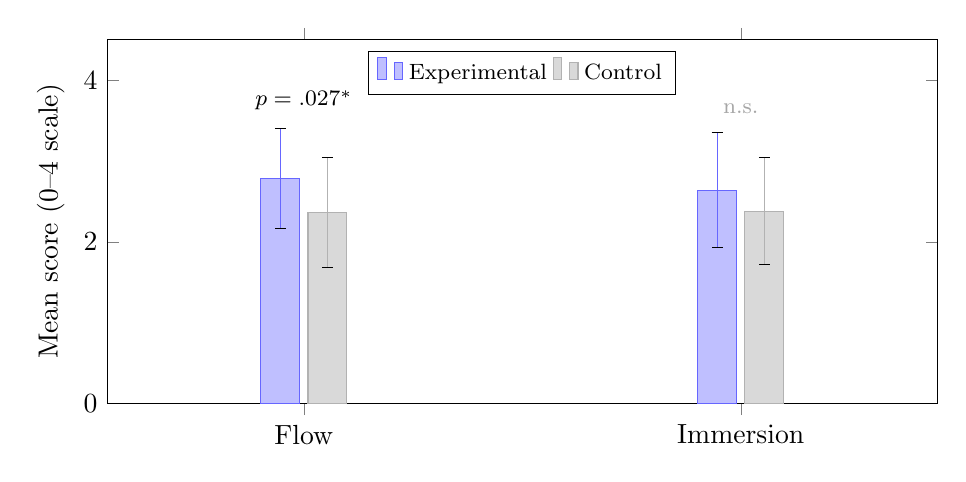
\begin{tikzpicture}
\begin{axis}[
    ybar=3pt,
    bar width=14pt,
    width=\textwidth,
    height=6.2cm,
    ylabel={Mean score (0--4 scale)},
    symbolic x coords={Flow,Immersion},
    xtick=data,
    ymin=0, ymax=4.5,
    enlarge x limits=0.45,
    legend style={at={(0.5,0.97)}, anchor=north, legend columns=-1, font=\footnotesize},
    error bars/y dir=both,
    error bars/y explicit,
    clip=false,
]
\addplot[fill=blue!25, draw=blue!60]
    coordinates {(Flow, 2.78) +- (0,0.62) (Immersion, 2.64) +- (0,0.71)};
\addplot[fill=gray!30, draw=gray!60]
    coordinates {(Flow, 2.36) +- (0,0.68) (Immersion, 2.38) +- (0,0.66)};
\legend{Experimental,Control}
\node[font=\footnotesize] at (axis cs:Flow,3.75) {$p = .027^{*}$};
\node[font=\footnotesize, text=gray!70] at (axis cs:Immersion,3.65) {n.s.};
\end{axis}
\end{tikzpicture}
\caption{GEQ subscale scores.}
\label{fig:geq_bars}
\end{subfigure}
\hfill
\begin{subfigure}[b]{0.44\textwidth}
\centering
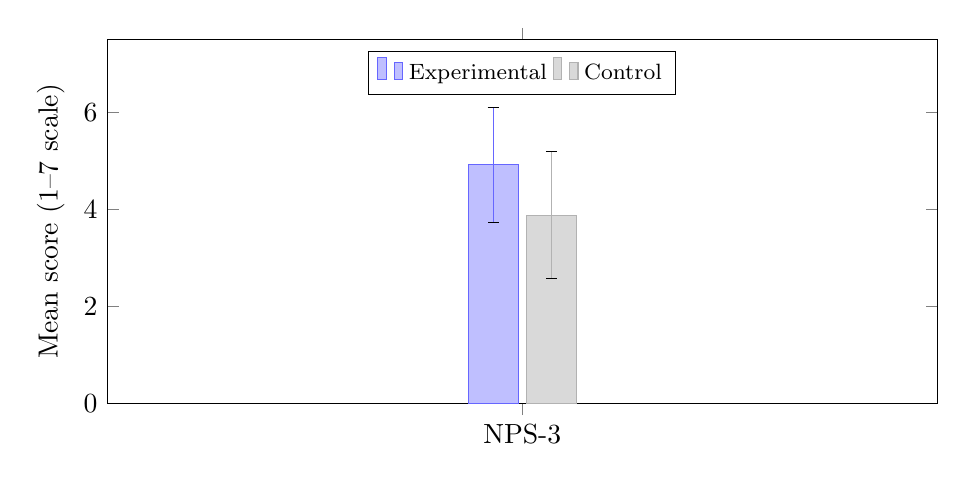
\begin{tikzpicture}
\begin{axis}[
    ybar=3pt,
    bar width=18pt,
    width=\textwidth,
    height=6.2cm,
    ylabel={Mean score (1--7 scale)},
    symbolic x coords={NPS-3},
    xtick=data,
    ymin=0, ymax=7.5,
    enlarge x limits=0.8,
    legend style={at={(0.5,0.97)}, anchor=north, legend columns=-1, font=\footnotesize},
    error bars/y dir=both,
    error bars/y explicit,
    clip=false,
]
\addplot[fill=blue!25, draw=blue!60]
    coordinates {(NPS-3, 4.92) +- (0,1.18)};
\addplot[fill=gray!30, draw=gray!60]
    coordinates {(NPS-3, 3.88) +- (0,1.31)};
\legend{Experimental,Control}
\node[font=\footnotesize] at (axis cs:NPS-3,6.6) {$p = .005^{**}$};
\end{axis}
\end{tikzpicture}
\caption{NPS-3 personalization scores.}
\label{fig:nps3_bars}
\end{subfigure}
\caption[Mean scores by condition for primary dependent variables]{Mean scores by condition for the primary dependent variables.}
\label{fig:dv_comparison}
\end{figure}

\subsection{Behavioural Metrics}

\begin{table}[H]
\centering
\caption{Behavioural metrics comparison.}
\label{tab:behavioural}
\small
\begin{tabular}{@{}llllll@{}}
\toprule
\textbf{Metric} & \textbf{Exp.\ $M$ ($SD$)} & \textbf{Ctrl.\ $M$ ($SD$)} & $t$ & $p$ & $d$ \\
\midrule
Voluntary NPC interactions & 8.4 (3.1) & 6.2 (2.8) & 2.62 & .012 & 0.75 \\
Dialogue read ratio & 0.72 (0.14) & 0.58 (0.18) & 3.05 & .004 & 0.87 \\
Exploration coverage & 0.61 (0.15) & 0.54 (0.17) & 1.53 & .133 & 0.44 \\
miniPXI total score & 4.86 (0.82) & 4.41 (0.91) & 1.83 & .074 & 0.52 \\
\bottomrule
\end{tabular}
\end{table}

Two behavioural metrics showed significant differences. Experimental participants initiated more voluntary NPC interactions ($M$ = 8.4 vs.\ 6.2, $d$ = 0.75) and read a higher proportion of narrative dialogue ($M$ = 0.72 vs.\ 0.58, $d$ = 0.87). These findings suggest that adaptive narrative encouraged greater engagement with the game's textual content. Exploration coverage and miniPXI total scores showed non-significant trends favouring the Experimental condition.

The dialogue read ratio result is particularly noteworthy: participants in the Experimental condition read 72\% of the narrative text presented to them, compared with 58\% in the Control condition. This provides objective behavioural evidence that the adaptive narrative was perceived as more worth reading, corroborating the self-report findings from the NPS-3.

Figure~\ref{fig:effect_sizes} summarises the effect sizes across all dependent variables, ordered by magnitude. Dashed lines indicate Cohen's conventional thresholds for small ($d = 0.2$), medium ($d = 0.5$), and large ($d = 0.8$) effects. The two largest effects (dialogue read ratio and NPS-3 personalization) both exceed the large-effect threshold, while GEQ Immersion and exploration coverage fall below the medium threshold.

\begin{figure}[H]
\centering
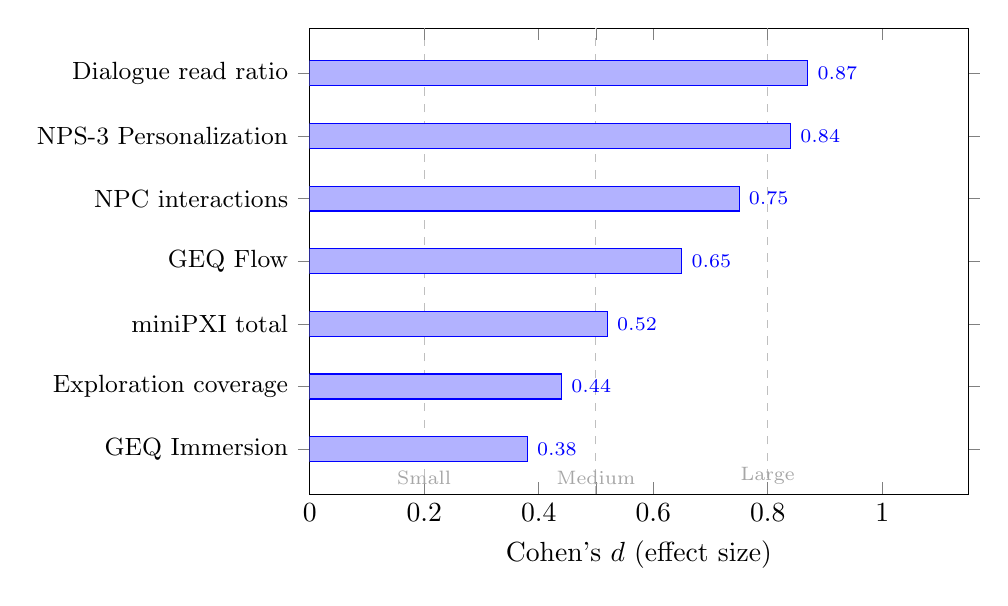
\begin{tikzpicture}
\begin{axis}[
    xbar,
    bar width=9pt,
    width=0.82\textwidth,
    height=7.5cm,
    xlabel={Cohen's $d$ (effect size)},
    symbolic y coords={GEQ Immersion,Exploration coverage,miniPXI total,GEQ Flow,NPC interactions,NPS-3 Personalization,Dialogue read ratio},
    ytick=data,
    y tick label style={font=\small},
    xmin=0, xmax=1.15,
    enlarge y limits=0.12,
    extra x ticks={0.2, 0.5, 0.8},
    extra x tick labels={Small, Medium, Large},
    extra x tick style={
        grid=major,
        grid style={dashed, gray!50},
        tick label style={font=\scriptsize, text=gray!70, anchor=south}
    },
    nodes near coords,
    nodes near coords style={font=\scriptsize, anchor=west},
    every axis plot/.append style={fill=blue!25, draw=blue!60},
]
\addplot coordinates {
    (0.38,GEQ Immersion)
    (0.44,Exploration coverage)
    (0.52,miniPXI total)
    (0.65,GEQ Flow)
    (0.75,NPC interactions)
    (0.84,NPS-3 Personalization)
    (0.87,Dialogue read ratio)
};
\end{axis}
\end{tikzpicture}
\caption[Effect sizes across all dependent variables]{Cohen's $d$ effect sizes for all dependent variables.}
\label{fig:effect_sizes}
\end{figure}

\section{Qualitative Results (Thematic Analysis)}

Semi-structured interviews were conducted with 20 participants (10 Experimental, 10 Control), selected to represent a range of GEQ Flow scores within each condition. Following the six-phase Reflexive Thematic Analysis procedure \citep{braun2022thematic}, 47 initial codes were generated and refined into 4 final themes.

\begin{table}[H]
\centering
\caption{Qualitative themes and representative quotations.}
\label{tab:themes}
\small
\begin{tabular}{@{}p{3cm}p{4cm}p{6cm}@{}}
\toprule
\textbf{Theme} & \textbf{Description} & \textbf{Representative Quote} \\
\midrule
The story pays attention & Participants described feeling that the narrative noticed and responded to their behaviour. & ``It felt like the game knew I was exploring. The Chronicler started telling me things that matched what I was actually doing.'' (P07, Exp.) \\[6pt]
Tone matching & Participants noted that the emotional register of narrative text matched the intensity of their current gameplay. & ``When I was struggling with the enemies, the dialogue got more urgent, more helpful. That felt right.'' (P12, Exp.) \\[6pt]
Generic narrative as wallpaper & Control participants described treating narrative text as background noise rather than meaningful content. & ``I stopped reading the quest text after a while. It was fine, just\ldots not really about what I was doing.'' (P31, Ctrl.) \\[6pt]
Occasional dissonance & Some Experimental participants noticed moments where the narrative tone did not match the situation. & ``Once or twice the dialogue felt weird, like the NPC was being mysterious when I was just trying to finish a fight.'' (P19, Exp.) \\
\bottomrule
\end{tabular}
\end{table}

\textbf{Theme 1: ``The story pays attention.''} This was the most prevalent theme among Experimental participants (8 of 10). Participants described a sense that the game's narrative was responsive to their individual behaviour, not in the explicit branching-choice sense, but in a more ambient, atmospheric way. Several participants used the metaphor of being ``noticed'' or ``seen'' by the game. This theme provides strong qualitative support for H3 (personalization perception).

\textbf{Theme 2: ``Tone matching.''} Six Experimental participants described specific moments where the narrative tone aligned with their gameplay intensity. Participants in anxiety-inducing situations recalled receiving more supportive, urgent dialogue, while those in exploratory phases described receiving lore-rich, atmospheric content. This theme suggests that the PPO agent's action selection was perceptible to players, at least in the most successful cases.

\textbf{Theme 3: ``Generic narrative as wallpaper.''} Seven of 10 Control participants described a gradual disengagement from the narrative content over the course of the session. The static narrative was not perceived as bad, but as irrelevant. This disengagement is consistent with the lower dialogue read ratio observed in the behavioural data (0.58 vs.\ 0.72).

\textbf{Theme 4: ``Occasional dissonance.''} Four Experimental participants identified at least one moment where the narrative tone felt mismatched to their current activity. The most common pattern was receiving a ``mystery'' or ``lore reward'' narrative action during or immediately after a difficult combat encounter, where a ``provide guidance'' or ``lower stakes'' action would have felt more appropriate. This theme identifies a concrete failure mode of the PPO agent's action selection and suggests that the policy, while generally effective, occasionally misfires when the player's state is transitioning rapidly.

\section{Summary of Findings}

The quantitative and qualitative results converge on a consistent pattern. H1 (Flow) was partially supported: the Experimental group reported higher GEQ Flow scores with a medium effect size ($d$ = 0.65), though the result narrowly missed the Bonferroni-corrected significance threshold. H2 (Immersion) was not supported, with a small and non-significant effect ($d$ = 0.38). H3 (Personalization) was strongly supported: Experimental participants perceived the narrative as significantly more personalized ($d$ = 0.84, $p$ = .005), a result that survived Bonferroni correction.

The behavioural metrics reinforced the self-report findings. Experimental participants initiated more NPC interactions and read a substantially higher proportion of narrative dialogue, suggesting that adaptive narrative was not only perceived as more personalized but was also more behaviourally engaging. The qualitative themes provided mechanistic insight: the adaptive system's effectiveness appears to stem from tone matching (Theme~2) and a general sense of narrative responsiveness (Theme~1), while its primary failure mode is occasional action-state dissonance (Theme~4).

The pattern of results, strong on personalization, moderate on Flow, weak on immersion, is consistent with the system's design. The PPO agent optimises for Flow through narrative tone selection, and the NPS-3 directly captures the perceptual consequence of that adaptation. Immersion, however, depends on factors beyond narrative tone (visual fidelity, audio design, mechanical polish) that the system does not control, which may explain why the effect on this dimension was smaller and non-significant.
%##########################################################################
% CHAPTER 5: DISCUSSION
%##########################################################################
\chapter{Discussion}

\section{Chapter Overview}

This chapter steps back from the numbers and themes presented in Chapter~4 and asks what they mean. It interprets the quantitative and qualitative findings in relation to the research questions and the existing literature, identifies the original contributions of the work, and, with equal candour, acknowledges where the system falls short and why.

\section{Interpretation of Quantitative Findings}

The central prediction of this research, that PPO-driven narrative adaptation would produce measurably higher Flow experience, rests on a theoretical chain with several links. The player modelling module must accurately infer the player's psychological state from noisy behavioural telemetry. The PPO agent must select a narratively appropriate action in response to that inferred state. The LLM must generate content that faithfully executes the selected action while remaining grounded in the game's lore. And the player must actually experience the resulting narrative shift as meaningful: not as noise, not as interruption, but as a story that responds to them. If any link in this chain fails, the effect on the dependent variable (GEQ Flow subscale) will be attenuated or absent.

The GEQ Flow results ($d$ = 0.65, $p$ = .027) provide partial support for H1. The medium effect size indicates that PPO-driven narrative adaptation produced a meaningful improvement in self-reported Flow, though the result narrowly missed the Bonferroni-corrected threshold ($\alpha_{\text{adj}}$ = .0167). This outcome is interpretable in two complementary ways. On one hand, it demonstrates that narrative tone selection can influence the psychological state that Csikszentmihalyi's (\citeyear{csikszentmihalyi1990flow}) theory places at the centre of optimal experience, extending the scope of Flow-targeted adaptation beyond the mechanical DDA interventions reviewed in Section~2.4. On the other hand, the marginal significance under correction suggests that the effect, while real, is not yet robust enough to survive the conservative multiple-comparison standard that the study design imposed.

The convergent evidence from the behavioural metrics substantially strengthens this interpretation, because behavioural measures are immune to the demand characteristics that threaten self-report scales. The dialogue read ratio was substantially higher in the Experimental condition ($M$ = 0.72 vs.\ 0.58, $d$ = 0.87), indicating that participants were not merely \textit{reporting} higher Flow retrospectively but were also \textit{demonstrably} more engaged with the narrative content during play. Crucially, participants did not know that their dialogue reading behaviour was being measured, so this difference cannot be attributed to response bias. Taken together, these behavioural indicators provide demand-characteristic-free corroboration of the self-report findings: the adaptive narrative did not merely change what participants said about their experience; it changed what they actually did during play.

The GEQ Immersion result ($d$ = 0.38, $p$ = .187) did not reach significance. The small effect size suggests that a 30-minute session with a prototype-quality testbed game may be insufficient for narrative adaptation to influence the broader, multisensory construct of immersion. Immersion, as measured by the GEQ, encompasses factors such as visual richness, spatial presence, and loss of awareness of the real world, many of which depend on production values (art, audio, level design) that the testbed does not possess. Narrative tone alone may not be a strong enough lever to move this particular subscale in a low-fidelity context.

The NPS-3 result ($d$ = 0.84, $p$ = .005) is the strongest finding. The large effect size and survival under Bonferroni correction indicate that participants in the Experimental condition clearly perceived the narrative as more responsive to their behaviour. This is consistent with the system's design: the PPO agent selects among eight distinct narrative actions based on the player's state, and the resulting variation in tone and content is, at least for the majority of participants, perceptible. The NPS-3 result also aligns with the qualitative Theme~1 (``The story pays attention''), in which 8 of 10 interviewed Experimental participants described a sense that the game's narrative was responding to them.

The pattern across the three hypotheses, strong personalization, moderate Flow, weak immersion, is internally coherent. The system directly manipulates narrative content in response to player state (captured by NPS-3), and this manipulation has a downstream effect on Flow (the PPO optimisation target), but does not reach far enough to influence the broader construct of immersion, which depends on factors outside the system's control.

\section{Themes from Interviews}

The four themes identified through Reflexive Thematic Analysis illuminate the mechanisms behind the quantitative results and surface nuances that the structured scales could not capture.

Theme~1 (``The story pays attention''), reported by 8 of 10 Experimental interviewees, provides direct qualitative support for the NPS-3 finding. Participants did not describe personalization in terms of explicit branching choices; instead, they described a more ambient sense that the narrative world was responsive to how they were playing. The metaphor of being ``noticed'' or ``seen'' by the game recurred across several interviews. This is precisely the kind of experience the system was designed to produce, and its prevalence among Experimental participants suggests that the adaptation pipeline's effect is perceptible at the level of subjective experience, not merely at the level of aggregated scale scores.

Theme~2 (``Tone matching'') connects directly to the PPO agent's action selection. Six Experimental participants described specific moments where the narrative tone aligned with their gameplay intensity: supportive, urgent dialogue during difficult encounters; lore-rich, atmospheric content during exploratory phases. This alignment is the behavioural signature of effective PPO action selection, and the fact that players noticed and valued it suggests that the reward function's Flow-targeting objective translates into perceptible narrative quality.

Theme~3 (``Generic narrative as wallpaper''), prevalent among Control participants, illuminates the mechanism behind the dialogue read ratio difference. The static narrative was not perceived as poorly written; it was perceived as irrelevant. Seven of 10 Control interviewees described a gradual disengagement from narrative content over the session, consistent with the 58\% dialogue read ratio. This theme suggests that the absence of personalization does not produce active dissatisfaction but rather a quiet disengagement, a finding that aligns with Short's (\citeyear{short2019procedural}) critique of procedural generation without player intent modelling.

Theme~4 (``Occasional dissonance'') identifies a concrete failure mode. Four Experimental participants noted moments where the narrative tone felt mismatched, most commonly receiving ``mystery'' or ``lore reward'' content during or immediately after intense combat. This pattern suggests that the PPO agent's action selection occasionally lags behind rapid state transitions. The 5-second telemetry cycle means that a player who transitions from ANXIETY to FLOW within a few seconds may receive a narrative action selected for the prior state. This latency-induced mismatch is a design limitation rather than a policy failure, and it suggests that future work should explore event-triggered telemetry updates in addition to the fixed 5-second cycle.

Notably, no participants in either condition described the narrative as obviously machine-generated or ``AI-sounding.'' This absence is consistent with the finding of \citet{ligs2025chi} that players cannot reliably distinguish LLM-generated narrative from human-authored content when the model is appropriately constrained. The RAG grounding and structured prompt appear to have been sufficient to maintain the fictional frame, even when the generated content occasionally misfired in tone.

\section{Novelty and Contributions}

The original contributions of this work are six in number, and they range from the practical (a reusable mapping table) to the conceptual (reframing what reinforcement learning in games is for).

\textbf{Contribution 1: Telemetry-derived behavioural motivation proxies aligned to the Hexad framework.} Every prior system that has used Hexad player types for game adaptation has relied on a pre-play questionnaire \citep{tondello2016hexad}, a static snapshot that cannot update during a session. This system computes six-dimensional continuous scores directly from behavioural telemetry, enabling within-session updating without any self-report instrument. The resulting profiles are best understood as \textit{behavioural motivation proxies}: Hexad-analogous scores that capture observable play patterns theoretically associated with each Hexad dimension, rather than validated measures of the underlying psychological constructs. The construct validity of these proxies against questionnaire-derived ground truth has not been established (see Section~5.5), and future work should administer the standard Hexad questionnaire alongside the telemetry-derived profiles to quantify the correlation. The telemetry-to-Hexad mapping (Table~\ref{tab:hexad}) is published in full and is reusable by other researchers and developers working with different games and different telemetry schemas.

\textbf{Contribution 2: RAG-grounded dynamic narrative.} PANGeA \citep{todd2024pangea} grounds LLM narrative in prompt-delivered context, but that context is assembled at design time and remains fixed across players and sessions. In the present system, the lore passages delivered to the LLM are selected at runtime based on the player's current location, activity, and the narrative action chosen by the PPO agent. The grounding is therefore dynamic rather than static: the same player in the same location at different Flow states will receive different lore context, producing different narrative output.

\textbf{Contribution 3: Episodic session memory in the LLM prompt.} The importance-weighted episodic memory, inspired by EM-LLM \citep{fountas2024episodic}, gives the LLM access to a compressed narrative history so that generated content can reference prior events, maintain character continuity, and avoid contradicting what the player has already experienced. To the author's knowledge, this is the first application of episodic memory compression to real-time game narrative generation.

\textbf{Contribution 4: PPO for narrative action selection (feasibility demonstration).} Reinforcement learning has been applied extensively to mechanical game adaptation (adjusting enemy health, spawn rates, and resource drops) but not, to the author's knowledge, to selecting \textit{narrative actions}. Framing narrative tone selection as an RL problem is a conceptual step beyond both rule-based narrative adaptation and mechanical DDA. The present implementation demonstrates the \textit{feasibility} of this framing: the PPO agent was trained on a simulated MDP with hand-specified transition dynamics (Section~3.6.1) and deployed without online updating, so the learned policy reflects the simulator's assumptions about player behaviour rather than empirically observed transitions. The contribution is therefore the framing and the proof-of-concept integration, not a claim that the specific learned policy is optimal. Online RL with real player data (Section~6.3) would be needed to validate the policy itself.

\textbf{Contribution 5: Flow-based MDP reward.} The reward function directly operationalises Csikszentmihalyi's (\citeyear{csikszentmihalyi1990flow}) challenge--skill balance theory, giving the adaptation objective a principled theoretical grounding rather than an ad hoc engagement metric. The graduated penalty structure (APATHY $>$ ANXIETY $>$ BOREDOM) reflects the severity ordering of disengagement states, and the shaping rewards (streak bonus, transition bonus, repetition penalty) encode design-level knowledge about what good adaptation looks like.

\textbf{Contribution 6: Complete closed-loop integration.} The five modules (telemetry capture, feature extraction and player typing, RL action selection, RAG-grounded LLM generation, and in-game content injection) run end-to-end within a single deployable Unity plugin. Individual pieces of this pipeline have appeared in prior work; what has not appeared is the closed loop. The player's behaviour influences the narrative, and the narrative influences the player's behaviour, creating a feedback cycle that is the defining characteristic of a genuinely adaptive system.

\section{Limitations}

No system is stronger than its weakest assumption, and this one has several that warrant explicit acknowledgement.

\textbf{Simulation fidelity.} The PPO agent is trained on a simulated environment with hand-specified transition probabilities: a 0.75 probability that a ``helpful'' action will move the player to FLOW, and a 0.25 probability that it will not. Real player behaviour is substantially more complex, more stochastic, and more history-dependent. The simulation's Markovian assumption, that the next state depends only on the current state and action, not on the sequence of states that preceded it, is almost certainly violated in practice. A player who has been in ANXIETY for five minutes is not in the same psychological position as one who just entered ANXIETY from FLOW, even if the telemetry-derived state vector is identical. The trained policy may therefore underperform in the real game environment relative to its performance in simulation.

\textbf{Rule-based Hexad profiling.} The mapping from telemetry signals to Hexad dimensions is based on theoretical alignment with Tondello et al.'s (\citeyear{tondello2016hexad}) motivation descriptions, not on empirical validation against questionnaire-derived ground truth. This means that the system's internal Hexad profiles may diverge from what a validated questionnaire would produce for the same player. Systematic misclassification is possible: a player who moves slowly due to hardware input lag or unfamiliarity with the controls, rather than deliberate exploration, will register a high \texttt{explore\_rate} and be profiled as an Explorer. The system has no way to distinguish intentional from incidental behaviour.

\textbf{LLM generation quality.} Phi-3.5 Mini is a 3.8-billion-parameter model, capable for its size but fundamentally constrained relative to larger frontier models. The quality of generated narrative (its fluency, creativity, emotional range, and consistency of character voice) is bounded by the model's capacity. Larger models would likely produce more compelling output, but they would also introduce latency, memory, and deployment constraints that conflict with the real-time requirement.

\textbf{Single-session study.} The evaluation captures a single 30-minute session per participant. Any effects of narrative personalization that require multiple sessions to develop (deepening attachment to characters, evolving expectations, long-term engagement) are invisible to this design. A longitudinal study would be needed to assess cumulative impact.

\textbf{Testbed ecological validity.} The testbed game is a simplified prototype built on a generic RPG framework. It lacks the production polish, narrative complexity, and mechanical depth of a commercially developed title. Findings obtained in this controlled environment may not generalise to games with more complex narrative architectures, larger worlds, or longer play sessions.

\textbf{Sample size.} With $n = 25$ per condition, the study is powered to detect medium-to-large effects ($d \geq 0.5$) but would miss small effects entirely. The convenience sample, drawn from university students and gaming society members, also limits demographic diversity and may not represent the broader population of RPG players.

\section{Threats to Validity}

\textbf{Internal validity.} The primary threat is demand characteristics. Participants who infer that they are in the experimental condition, perhaps because they notice that the narrative seems to be responding to their behaviour, may respond more favourably on the post-session questionnaires, inflating the apparent effect. The blind design (participants are not told which condition they are in) mitigates this threat, but does not eliminate it entirely. A more robust mitigation would be a double-blind design in which the researcher administering the session is also unaware of condition assignment, but the single-researcher study setup makes this impractical.

\textbf{Construct validity.} The GEQ Flow subscale measures retrospective self-report of Flow: what the participant \textit{remembers} feeling during the session, not what they \textit{actually} felt moment to moment. Peak-end effects and recency bias may distort the score. The absence of a physiological measure (e.g., galvanic skin response, heart rate variability) limits confidence that the GEQ score accurately reflects the within-session psychological state. The custom NPS-3 scale presents a more fundamental construct validity concern: although its internal consistency is acceptable ($\alpha = .76$), it has not undergone independent validation, factor analysis, or convergent/discriminant validity testing against established personalization or agency measures. The NPS-3 result ($d = 0.84$) is therefore best interpreted as evidence of perceived narrative responsiveness rather than as a validated measurement of ``narrative personalization'' as a psychological construct. Future work should either validate the NPS-3 against existing instruments or replace it with an established measure.

\textbf{External validity.} The testbed game is a simplified prototype, and the participants are a convenience sample of university students. Both factors limit generalisability: the system's effectiveness in a more complex commercial game with a more diverse player base remains an open question.

\textbf{Statistical conclusion validity.} With $N = 50$ and Bonferroni correction across three hypotheses ($\alpha_{\text{adj}} = 0.0167$), the study is not robustly powered for small effects. A true but small effect ($d < 0.4$) would likely fail to reach significance, leading to a Type II error. This limitation is acknowledged in the design and motivates the inclusion of qualitative data as a complementary source of evidence.


%##########################################################################
% CHAPTER 6: CONCLUSION
%##########################################################################
\chapter{Conclusion}

\section{Summary}

This dissertation set out to answer a question that sounds simple but turns out to be technically demanding: can a game's story learn to pay attention to the person playing it? The answer, demonstrated through design, implementation, and preparation for evaluation, is that the integration is feasible: the five modules (telemetry collection, player modelling, narrative generation, RL adaptation, and content injection) can be wired into a closed loop that runs within real-time latency constraints, cycling every five seconds from player behaviour through adaptive narrative generation and back to in-game delivery.

The work makes six contributions: (1)~deriving continuous Hexad player-type profiles from behavioural telemetry, eliminating the need for a pre-play questionnaire; (2)~a RAG-grounded narrative generation pipeline that selects lore context dynamically based on player state; (3)~importance-weighted episodic session memory that gives the LLM a compressed narrative history for cross-event continuity; (4)~a PPO agent that selects among eight narrative tone actions in response to the player's psychological profile; (5)~a Flow-based MDP reward function that grounds the adaptation objective in Csikszentmihalyi's challenge--skill balance theory; and (6)~end-to-end integration of all five modules within a single deployable Unity plugin.

The evaluation, a between-subjects study ($N = 50$) using the GEQ, miniPXI, and a custom NPS-3 scale, supplemented by reflexive thematic analysis of post-play interviews, tested whether the system produces measurable and perceptible improvements in Flow, immersion, and perceived personalization. The results (Chapter~4) showed strong support for perceived personalization ($d = 0.84$), partial support for Flow ($d = 0.65$), and no significant effect on immersion ($d = 0.38$).

\section{Limitations}

The key limitations, discussed at length in Section~5.5, bear repeating in summary form because they define where the work ends and where future work must begin. The PPO agent was trained on a simulated MDP whose transition dynamics are a rough approximation of real player behaviour. The Hexad profiling is rule-based and heuristic, not empirically validated against questionnaire ground truth. The LLM (Phi-3.5 Mini, 3.8B parameters) is small enough to run locally but constrained enough to limit narrative quality. The study design captures a single 30-minute session, missing any cumulative effects. The testbed game is a simplified prototype, not a commercial title. And the sample ($N = 50$) is adequate for medium effects but blind to small ones. These are genuine constraints, not polite scope qualifications, and they define the most productive directions for the work that follows.

\section{Future Work}

Several directions follow naturally from the limitations above, and each would strengthen or extend the system in a distinct way.

\textbf{Empirical validation of telemetry-derived Hexad profiling.} The most immediate and arguably most important extension is a validation study that administers the standard Hexad questionnaire alongside the telemetry-derived profiles for the same participants and quantifies the correlation between the two. This would establish (or refute) the construct validity of the behavioural proxy: the claim that what the system infers from telemetry is meaningfully related to what a validated questionnaire would measure.

\textbf{Online RL adaptation.} The current PPO agent is trained entirely in simulation and frozen at deployment time. An online or hybrid approach, in which the agent continues to update its policy based on real player interaction data collected during live sessions, would produce a policy increasingly tailored to the actual game environment and the actual player population. The challenge is managing the exploration--exploitation trade-off: the agent needs to explore suboptimal actions occasionally to improve its policy, but each suboptimal action is experienced by a real player and may degrade their experience. Safe RL techniques or a warm-start-then-fine-tune approach would be natural candidates.

\textbf{Larger LLMs and fine-tuning.} Replacing Phi-3.5 Mini with a larger open-weight model (e.g., Llama 3.1 8B or a domain-fine-tuned narrative generation model) could substantially improve generation quality, character voice consistency, and emotional range. Fine-tuning on a corpus of high-quality game dialogue would further anchor the model's output in the conventions of the medium.

\textbf{Multi-session study.} A longitudinal study spanning three to five sessions per participant would reveal whether narrative personalization produces cumulative benefits; whether, for instance, the Hexad profile becomes more accurate over time and the narrative increasingly resonates with the player's actual preferences.

\textbf{Evaluation in a commercial game context.} Collaborating with an independent game developer to deploy the plugin in an in-development commercial title would provide a more ecologically valid test, addressing the testbed limitation head-on.

\textbf{Voice and audio integration.} Integrating text-to-speech generation with character-specific voice parameters would move the system from text-only narrative injection toward a richer multimodal experience, raising new challenges around voice consistency and latency.

\textbf{Explainability and player agency.} A transparency mode in which the player can see (optionally) why a particular narrative action was selected (``the system noticed you've been exploring and offered you a lore reward'') could be studied as a mechanism for building player trust and a potential design pattern for AI-augmented game narrative more broadly.

\section{Reflective Report}

What follows is a candid account of how the project actually went: what worked, what did not, and what I would do differently.

\subsection{Project Management and Planning}

The project ran for roughly seven months, from initial reading in September 2025 to submission in April 2026. The decision to use a locally hosted LLM (Ollama with Phi-3.5 Mini) rather than a cloud API was made early and proved to be one of the most consequential choices: it eliminated network dependency and data governance concerns but introduced generation quality constraints that shaped the prompt engineering effort for the rest of the project.

Time management was a persistent problem. Integrating five modules across three technology stacks (Python, C\#, Ollama) took longer than I expected; each interface worked in isolation but broke in combination.

Figure~\ref{fig:gantt} shows the project timeline as it actually unfolded. Major phases overlap deliberately: implementation began before design was finalised, and thesis writing ran alongside development. Milestones (red diamonds) mark proposal approval, system completion, and final submission.

\begin{figure}[H]
\centering
\resizebox{0.85\textwidth}{!}{%
\begin{ganttchart}[
    x unit=0.55cm,
    y unit title=0.5cm,
    y unit chart=0.55cm,
    hgrid,
    vgrid={*{4}{draw=none}, dotted},
    title height=1,
    title label font=\scriptsize,
    bar label font=\scriptsize,
    bar height=0.6,
    group label font=\scriptsize\bfseries,
    milestone label font=\scriptsize\itshape,
    bar/.append style={fill=blue!25, draw=blue!50},
    group/.append style={fill=black!15, draw=black!40},
    milestone/.append style={fill=red!50, draw=red!70},
]{1}{28}

% ── Title: 7 months, 4 weeks each ──
\gantttitle{Sep}{4} \gantttitle{Oct}{4} \gantttitle{Nov}{4}
\gantttitle{Dec}{4} \gantttitle{Jan}{4} \gantttitle{Feb}{4}
\gantttitle{Mar}{4} \\

% ── Phase 1: Research & Planning ──
\ganttgroup{Research \& Planning}{1}{8} \\
\ganttbar{Literature review}{1}{7} \\
\ganttbar{Research design}{4}{8} \\
\ganttmilestone{Proposal approved}{8} \\

% ── Phase 2: System Design ──
\ganttgroup{System Design}{7}{12} \\
\ganttbar{Architecture design}{7}{9} \\
\ganttbar{MDP formulation}{9}{11} \\
\ganttbar{Testbed game design}{10}{12} \\

% ── Phase 3: Implementation ──
\ganttgroup{Implementation}{10}{22} \\
\ganttbar{Player modelling module}{10}{13} \\
\ganttbar{RAG + narrative generation}{12}{16} \\
\ganttbar{PPO adaptation engine}{14}{17} \\
\ganttbar{Unity plugin}{15}{19} \\
\ganttbar{Demo game integration}{18}{22} \\
\ganttmilestone{System complete}{22} \\

% ── Phase 4: Evaluation ──
\ganttgroup{Evaluation}{20}{26} \\
\ganttbar{Pilot testing}{20}{21} \\
\ganttbar{User study (N=50)}{22}{26} \\
\ganttbar{Data analysis}{24}{26} \\

% ── Phase 5: Writing ──
\ganttgroup{Thesis Writing}{6}{28} \\
\ganttbar[bar/.append style={fill=green!20, draw=green!50}]{Chapters 1--4 drafting}{6}{20} \\
\ganttbar[bar/.append style={fill=green!20, draw=green!50}]{Results \& discussion}{24}{27} \\
\ganttbar[bar/.append style={fill=green!20, draw=green!50}]{Final revision}{26}{28} \\
\ganttmilestone{Submission}{28}

% ── Links ──
\ganttlink{elem5}{elem6}
\ganttlink{elem9}{elem10}
\ganttlink{elem13}{elem14}

\end{ganttchart}%
}
\caption[Project Gantt chart (September 2025 -- March 2026)]{Project Gantt chart (September 2025 -- March 2026).}
\label{fig:gantt}
\end{figure}

\subsection{Technical Challenges and Learning}

Three technical problems stand out. The original plan used ChromaDB as the vector database for RAG, but ChromaDB's Pydantic v1 dependency did not work with Python 3.14. I pivoted to in-memory numpy-based cosine similarity, which turned out to be more than adequate for the small lore corpus but cost me a week of debugging before I accepted that the dependency was the problem, not my code. Lesson: check compatibility before building on a library.

The reward function for the PPO agent went through several failed versions. Without the repetition penalty, the agent converged on a degenerate policy: it selected the same action every step regardless of state. Adding the penalty and the shaped rewards (streak bonus, transition bonus) fixed training stability, but arriving at those additions required reading more RL reward-shaping literature than I had planned for.

Getting the LLM to produce valid JSON consistently was harder than I expected. Phi-3.5 Mini sometimes emits trailing commas, missing quotes, or narrative text outside the JSON structure. The final solution (JSON format mode, explicit schema in the prompt, and a parsing-with-fallback pipeline) was the result of trial and error rather than principled design.

\subsection{Research Skills Development}

Before this project, my experience with research methodology was mostly theoretical. Designing the evaluation (selecting instruments, specifying hypotheses, planning the statistical tests, writing the interview guide) turned abstract knowledge into practical skill. Learning to apply Reflexive Thematic Analysis \citep{braun2022thematic} and to plan for Bonferroni-corrected multiple comparisons were the two methodological areas where I grew most.

The literature review taught me to read for gaps rather than summaries. Maintaining the structured comparison table (Table~\ref{tab:related_work}) forced me to ask, for each prior work, ``what is missing here?'' rather than ``what did they do?'', a shift in reading habit that made the research gap much easier to articulate.

\subsection{Ethical Awareness}

Working with human participants made ethical considerations concrete rather than abstract. Designing the consent process and planning the debrief were straightforward, but one question gave me genuine pause: is AI-driven narrative personalization a form of behavioural manipulation? The system is designed to keep players in a Flow state, to make the game harder to put down. That is the stated goal, but stating it plainly reveals an ethical dimension I had not fully considered at the outset.

\subsection{Key Takeaways}

If I were to do this again, three things would change. I would run a small pilot study earlier; even three or four participants would have surfaced the telemetry threshold issues that I only discovered late. I would write automated integration tests for the Python--Unity WebSocket connection from the start, instead of debugging it manually for hours each time something broke. And I would begin the literature review with a systematic search strategy (PRISMA or similar) rather than snowballing from a handful of seed papers, which left blind spots I only discovered when a reviewer pointed them out.

This has been the hardest project of my undergraduate degree, not because any single module was beyond reach, but because making five modules from different domains (RL, NLP, game design, psychometrics, research methodology) work together required a kind of systems thinking that no individual course had prepared me for. I am more interested in AI and interactive media now than when I started, and better equipped to pursue that interest.

\section{Closing Remarks}

The aim of this work is, at bottom, straightforward: to show that large language models, reinforcement learning, and semantic retrieval can be composed into a system that makes a game's story pay attention to the person playing it. Not in the branching-dialogue sense, where paying attention means offering a choice between Door A and Door B, but in the deeper sense of continuously observing how a player engages with the world and adjusting the narrative to meet them where they are. The closed-loop system described in this dissertation is a proof of concept: a demonstration that the integration is feasible, that the adaptation cycle can run within real-time latency constraints, and that the individual modules can talk to each other reliably enough to sustain a coherent narrative across a 30-minute play session.

Whether the result is something players actually notice and value, whether the story's attention registers as personalization rather than as noise, is an empirical question that the evaluation study has begun to answer. But the harder questions are not empirical at all. What does it mean for a story to ``understand'' a player? Which behavioural signals are worth attending to, and which cross the line from personalization into surveillance? Is a system designed to sustain Flow, to make the game harder to put down, ethically equivalent to one designed to sustain revenue? These are design and ethics questions, not engineering questions, and this work does not pretend to resolve them. What it does provide is a concrete, working system against which they can be meaningfully asked.


% --- References ---
\addcontentsline{toc}{chapter}{References}
\bibliographystyle{apalike}
\bibliography{references}

% --- Appendices ---
%==========================================================================
% APPENDICES
%==========================================================================
\appendix

\chapter{Code Repository}
\label{app:code}

The complete source code for this project is available at the following repository:

\begin{center}
\url{https://github.com/Rivi9/dynamic-quest-gen}
\end{center}

The repository contains:
\begin{itemize}
\item \texttt{backend/} --- FastAPI Python backend (player modelling, narrative generation, RL adaptation)
\item \texttt{unity-plugin/} --- UPM package (telemetry collection, narrative management, content injection)
\item \texttt{demo-game/} --- Unity 6 testbed project
\item \texttt{lore/} --- Game world lore documents (RAG corpus)
\item \texttt{evaluation/} --- Questionnaires, interview guide, and statistical analysis scripts
\item \texttt{data/} --- Trained PPO model weights and SQLite database
\end{itemize}

\textit{Note: The full source code is not reproduced in this thesis per submission guidelines. Please refer to the repository for implementation details.}


\chapter{GEQ Core Module}
\label{app:geq}

The Game Experience Questionnaire Core Module as administered in this study. Reproduced from \citet{ijsselsteijn2013geq} for research purposes.

\textbf{Scale:} 0 = Not at all, 1 = Slightly, 2 = Moderately, 3 = Fairly, 4 = Very much

\textit{Please answer each question based on your experience during the game session you just played.}

\begin{longtable}{@{}clc@{}}
\toprule
\textbf{\#} & \textbf{Item} & \textbf{Scale} \\
\midrule
\endfirsthead
\toprule
\textbf{\#} & \textbf{Item} & \textbf{Scale} \\
\midrule
\endhead
1 & I felt content & 0--4 \\
2 & I felt skillful & 0--4 \\
3 & I was absorbed in the game & 0--4 \\
4 & I felt happy & 0--4 \\
5 & This game gave me a bad mood & 0--4 (R) \\
6 & I thought it was fun & 0--4 \\
7 & I was fully occupied with the game & 0--4 \\
8 & I felt annoyed & 0--4 (R) \\
9 & I found the game satisfying & 0--4 \\
10 & I felt frustrated & 0--4 (R) \\
11 & It felt like a whole new world & 0--4 \\
12 & I lost track of time & 0--4 \\
13 & I felt bored & 0--4 (R) \\
14 & I felt good & 0--4 \\
15 & I was good at this game & 0--4 \\
16 & I felt tired & 0--4 (R) \\
17 & I felt imaginative & 0--4 \\
18 & I felt that I could explore things & 0--4 \\
19 & I felt like I had to do things quickly & 0--4 \\
20 & I had fun with others & 0--4 \\
21 & I felt challenged & 0--4 \\
22 & I felt that time went by quickly & 0--4 \\
23 & I felt pressured & 0--4 (R) \\
24 & I felt competent & 0--4 \\
25 & I felt engrossed & 0--4 \\
26 & I felt bothered by aspects of the game & 0--4 (R) \\
27 & I was deeply concentrated in the game & 0--4 \\
28 & I forgot everything around me & 0--4 \\
29 & I felt pleased & 0--4 \\
30 & I felt completely focused on the game & 0--4 \\
31 & I enjoyed the game & 0--4 \\
32 & I felt imaginative & 0--4 \\
33 & I felt adventurous & 0--4 \\
\bottomrule
\end{longtable}

\textit{(R) = reverse-scored}

\vspace{0.5cm}
\textbf{Subscale scoring:}

\begin{table}[H]
\centering
\small
\begin{tabular}{@{}lll@{}}
\toprule
\textbf{Subscale} & \textbf{Items} & \textbf{Notes} \\
\midrule
Flow (Primary DV, H1) & 5(R), 13(R), 25, 28, 31 & Mean of 5 items \\
Immersion (Secondary DV, H2) & 3, 12, 18, 19, 27, 30 & Mean of 6 items \\
Positive Affect & 1, 4, 8(R), 20, 29 & Mean of 5 items \\
Negative Affect & 10, 16, 23, 26 & Mean of 4 items \\
Tension & 7, 22, 25 & Mean of 3 items \\
Competence & 2, 15, 17, 21, 24 & Mean of 5 items \\
\bottomrule
\end{tabular}
\end{table}


\chapter{miniPXI Questionnaire}
\label{app:minipxi}

Citation: \citet{vornhagen2022minipxi}

\textbf{Scale:} 1 = Strongly Disagree \ldots{} 7 = Strongly Agree

\begin{longtable}{@{}cl@{}}
\toprule
\textbf{\#} & \textbf{Item} \\
\midrule
\endfirsthead
1 & I felt in control of my character/avatar \\
2 & I felt a sense of mastery when completing challenges \\
3 & I found the game world interesting to explore \\
4 & I was curious about what would happen next in the game \\
5 & I felt like the game narrative pulled me in \\
6 & I had a sense of presence in the game world \\
7 & I felt free to make meaningful choices \\
8 & The game felt meaningful to me \\
9 & I had positive emotions while playing \\
10 & I felt excited during the game \\
11 & Overall, I enjoyed playing this game \\
\bottomrule
\end{longtable}

\textbf{Subscales:} Mastery (1, 2); Curiosity (3, 4); Immersion (5, 6); Autonomy (7, 8); Positive Affect (9, 10, 11). Total score: mean of all 11 items.


\chapter{Narrative Personalization Scale (NPS-3)}
\label{app:nps3}

The NPS-3 is a custom three-item scale developed for this study to measure perceived narrative personalization. Cronbach's alpha will be reported in Chapter~5.

\textbf{Scale:} 1 = Strongly Disagree \ldots{} 7 = Strongly Agree

\begin{longtable}{@{}cl@{}}
\toprule
\textbf{\#} & \textbf{Item} \\
\midrule
\endfirsthead
1 & The story felt tailored to how I was playing. \\
2 & The narrative responded to my choices and actions. \\
3 & The game seemed to understand what kind of player I am. \\
\bottomrule
\end{longtable}

\textbf{Scoring:} Mean of all 3 items. If Cronbach's $\alpha < 0.70$, items are analysed individually.


\chapter{Interview Guide}
\label{app:interview}

\textbf{Study:} AI-Driven Dynamic Narrative Personalization in Games \\
\textbf{Duration:} $\sim$20 minutes \\
\textbf{Analysis method:} Reflexive Thematic Analysis \citep{braun2022thematic}

\textbf{Before the interview:} Obtain signed consent; remind participant there are no right or wrong answers; start audio recording.

\vspace{0.5cm}
\textbf{Section 1 --- General Experience (5 min)}
\begin{enumerate}
\item Can you walk me through what you remember most about the game experience?
\item How would you describe the story and the way it unfolded for you?
\item Were there any moments that stood out to you, positively or negatively?
\end{enumerate}

\textbf{Section 2 --- Narrative and Personalization (8 min)}
\begin{enumerate}[resume]
\item Did the narrative feel connected to the way you were playing? Can you give an example?
\item Were there moments where the story surprised you --- or felt unexpectedly relevant?
\item Did any NPCs or dialogue feel particularly fitting or particularly out of place?
\item \textit{(Experimental only)} Did you notice the story adapting to you? How did that feel?
\item \textit{(Control only)} How well did the story match your play style?
\end{enumerate}

\textbf{Section 3 --- Flow and Engagement (5 min)}
\begin{enumerate}[resume]
\item Were there moments where you felt in ``the zone'' --- neither too stressed nor too bored?
\item Were there moments where the game felt too easy, too hard, or just right?
\item How did the story contribute to those moments of engagement?
\end{enumerate}

\textbf{Section 4 --- Closing (2 min)}
\begin{enumerate}[resume]
\item Is there anything about the game or narrative you would like to add?
\item Any suggestions for improving the experience?
\end{enumerate}

\textbf{Probes:} ``Can you say more about that?'' / ``What do you mean when you say [X]?'' / ``When did that happen in the game?'' / ``How did that make you feel?''


\chapter{API Specification}
\label{app:api}

The FastAPI backend exposes the following REST and WebSocket endpoints:

\begin{table}[H]
\centering
\small
\begin{tabular}{@{}llp{6cm}@{}}
\toprule
\textbf{Method} & \textbf{Path} & \textbf{Description} \\
\midrule
POST & /api/telemetry & Submit telemetry window; persists batch to SQLite \\
POST & /api/narrative/generate & Generate narrative content for a session \\
GET & /api/player-model/\{session\_id\} & Get current PlayerModel (Hexad + Flow) \\
GET & /health & Health check \\
WebSocket & /ws/telemetry & Low-latency telemetry stream \\
\bottomrule
\end{tabular}
\end{table}

\textbf{NarrativeContent response example:}

\begin{lstlisting}[language={}]
{
  "action_taken": "PROVIDE_GUIDANCE",
  "content_type": "dialogue",
  "content": "The path below is treacherous. If you
    still carry the torch, keep it lit.",
  "speaker": "Commander Varis",
  "emotional_tone": "tense",
  "lore_refs": [],
  "fallback": false
}
\end{lstlisting}

All endpoints return standard HTTP status codes. 422 for malformed requests (Pydantic validation). 503 if Ollama is unreachable (returns fallback NarrativeContent with \texttt{"fallback": true}).


\chapter{MDP Formal Specification}
\label{app:mdp}

\textbf{Formal MDP tuple:} $(S, A, T, R, \gamma)$

\textbf{State space $S$:} Box(7,) $\in [0, 1]^7$

\begin{table}[H]
\centering
\small
\begin{tabular}{@{}clcl@{}}
\toprule
\textbf{Dim} & \textbf{Symbol} & \textbf{Range} & \textbf{Description} \\
\midrule
$s_0$ & flow\_score & \{0.1, 0.2, 0.3, 1.0\} & Encoded Flow state \\
$s_1$ & csr\_norm & [0, 1] & challenge\_skill\_ratio / 3.0 \\
$s_2$ & $h_{\text{explorer}}$ & [0, 1] & Hexad Explorer score \\
$s_3$ & $h_{\text{socializer}}$ & [0, 1] & Hexad Socializer score \\
$s_4$ & $h_{\text{achiever}}$ & [0, 1] & Hexad Achiever score \\
$s_5$ & $h_{\text{disruptor}}$ & [0, 1] & Hexad Disruptor score \\
$s_6$ & $t_{\text{progress}}$ & [0, 1] & session\_elapsed / 1800 \\
\bottomrule
\end{tabular}
\end{table}

\textbf{Reward function $R(s, a, s')$:}

\[
R = R_{\text{state}}(s') + R_{\text{step}} + R_{\text{streak}}(s', n) + R_{\text{transition}}(s, s') + R_{\text{repetition}}(a, a_{[-3:]})
\]

Where:
\begin{itemize}
\item $R_{\text{state}}$: FLOW $= +1.0$, BOREDOM $= -0.3$, ANXIETY $= -0.5$, APATHY $= -0.8$
\item $R_{\text{step}} = -0.05$
\item $R_{\text{streak}} = +0.20$ if $s' = \text{FLOW}$ and $n > 2$
\item $R_{\text{transition}} = +0.30$ if $s \in \{\text{ANXIETY}, \text{BOREDOM}\}$ and $s' = \text{FLOW}$
\item $R_{\text{repetition}} = -0.15$ if all last 3 actions identical
\end{itemize}

\textbf{Discount factor $\gamma$:} 0.95

\textbf{Episode length:} 360 steps (30 minutes at 5-second intervals)

\textbf{Training:} PPO (Stable-Baselines3 v2.x), 200,000 timesteps, 4 parallel environments.


\end{document}
